\documentclass[11pt,twoside]{article}

\usepackage[margin=1in]{geometry}
\usepackage{amsmath,amssymb,amsthm,mathtools}
\usepackage[inline,shortlabels]{enumitem}
\usepackage{booktabs}
\usepackage{xcolor}
\usepackage{microtype}
\usepackage{needspace}

% Revision date: maintained by scripts/build_lecture_notes.py. Keep this command.
\newcommand{\lecturerevised}{2026-10-05 21:23 UTC-06:00}
\usepackage{eso-pic}
\AddToShipoutPictureBG{%
  \AtPageLowerLeft{%
    \put(\LenToUnit{0.5\paperwidth},\LenToUnit{0.5in}){%
      \makebox(0,0){\normalfont\footnotesize\color{black!60}Last revised: \lecturerevised}%
    }%
  }%
}

\usepackage[square,authoryear]{natbib}
\usepackage[colorlinks=true,linkcolor=blue!60!black,
  urlcolor=blue!60!black,citecolor=blue!60!black]{hyperref}
\usepackage[nameinlink,capitalize]{cleveref}
\crefname{exercise}{Exercise}{Exercises}
\Crefname{exercise}{Exercise}{Exercises}
\hypersetup{pdftitle={Lecture 9: Interpolation and benign overfitting},
  pdfauthor={Csaba Szepesvari}}

\usepackage{../exercises/course-exercises}

\usepackage{enotez}
\DeclareInstance{enotez-list}{lecture}{list}{format=\normalsize,number={#1.}}
\setenotez{list-name=Endnotes,list-style=lecture,backref=true}
\crefname{endnote}{Endnote}{Endnotes}
\Crefname{endnote}{Endnote}{Endnotes}

\definecolor{courseblue}{HTML}{17365D}
\DeclareMathOperator{\trace}{tr}
\newcommand{\E}{\mathbb E}
\newcommand{\I}{\mathbb I}
\newcommand{\one}[1]{\I\{#1\}}
\renewcommand{\P}{\mathbb P}
\newcommand{\Law}{\mathcal L}
\newcommand{\R}{\mathbb R}
\newcommand{\KL}{D}
\newcommand{\TV}{\mathrm{TV}}
\newcommand{\suppmark}{\texorpdfstring{\textsuperscript{*}}{*}}
\makeatletter
\@for\@letter:=A,B,C,D,E,F,G,H,I,J,K,L,M,N,O,P,Q,R,S,T,U,V,W,X,Y,Z\do{%
  \expandafter\edef\csname c\@letter\endcsname{\noexpand\mathcal{\@letter}}}
\makeatother

\newtheorem{theorem}{Theorem}[section]
\newtheorem{proposition}[theorem]{Proposition}
\newtheorem{corollary}[theorem]{Corollary}
\newtheorem{lemma}[theorem]{Lemma}
\theoremstyle{definition}
\newtheorem{definition}[theorem]{Definition}
\newtheorem{example}[theorem]{Example}
\theoremstyle{remark}
\newtheorem{remark}[theorem]{Remark}
\newcommand{\ip}[1]{\langle #1 \rangle}
\renewcommand{\thepage}{9--\arabic{page}}
\renewcommand{\thesection}{9.\arabic{section}}
\renewcommand{\theequation}{9.\arabic{equation}}
\pagestyle{myheadings}
\markboth{Lecture 9: Interpolation and benign overfitting}
{Lecture 9: Interpolation and benign overfitting}

\begin{document}

\begin{center}
\fcolorbox{courseblue}{white}{%
\begin{minipage}{0.92\textwidth}
\vspace{1mm}
\textbf{CMPUT 654: Mathematical Foundations of Modern AI Systems}
\hfill Fall 2026

\vspace{3mm}
\begin{center}
{\Large\bfseries Lecture 9: Interpolation and benign overfitting}

\vspace{1mm}
October 1, 2026
\end{center}

\vspace{2mm}
\textit{Lecturer: Csaba Szepesv\'ari}
\hfill
\textit{Note prepared by: Csaba Szepesv\'ari}
\vspace{1mm}
\end{minipage}}
\end{center}

\noindent\textbf{Covered in class.}
The lecture opened with a brief discussion of the random-label experiments
of Zhang et al., which motivated the interpolation question. The main
development followed roughly \crefrange{sec:question}{sec:series}, up to
the statement of \cref{thm:weighted-legendre}; there was no time to prove
the theorem. The result for smooth functions in
\cref{cor:s-smooth-consistency} was also mentioned, and we discussed the
problem with expected risk and the use of clipping. The theorem's proof,
the kernel results, and the extended discussion of generalization theory
are supplementary material in these notes.

\medskip
\noindent\textbf{Reading guide.}
Motivated by exact fitting in large neural networks, these notes ask when
interpolation of noisy observations can coexist with consistent prediction.
We first determine how large the benign set can be by a point-correction
argument. We then use minimum-norm linear interpolation as a tractable proxy
for gradient training and analyze one polynomial procedure: Legendre
polynomials represent the low-degree signal, and bounded Chebyshev polynomials
provide the additional interpolation directions. Both are functions of the
same one-dimensional input. The main text derives the approximation and estimation bound;
\cref{app:legendre-proof} verifies its matrix assumptions.
\Cref{sec:minnorm,sec:interpretation} extend the discussion: they compare positive and
negative results for kernel interpolation and ask what they justify about
model size and training time. \Cref{sec:minnorm} first introduces kernels and
reproducing kernel Hilbert spaces through linear function approximation.
The optional discussion in \cref{sec:rethinking-generalization} examines
what the random-label experiments establish about generalization theory.
\Cref{app:expected-risk} explains why the polynomial guarantee in probability
does not control expected risk and how clipping repairs this failure.
The prerequisites are least squares, orthogonal projections, elementary
matrix algebra, and convergence in probability.
\Cref{app:l2-background} reviews the function-space terminology, and the
exercises ask you to supply the linear algebra used in the main proof.

\section{The question raised by interpolation}
\label{sec:question}

Large neural networks trained by gradient methods commonly reach zero training
error. In the experiments of \citet{zhang2017}, the same networks could also
fit arbitrarily randomized labels, while training on the original labels gave
useful test predictions. Thus the model and optimizer had enough capacity to
fit pure noise, yet exact fitting on the natural problem remained compatible
with prediction. This observation motivates the advice to use large models and
train them to interpolation. We ask when that advice describes a sound
statistical procedure.

We begin with a one-dimensional regression analogue. Suppose that
\[
 Y_i=f^\star(X_i)+\varepsilon_i,
 \qquad \E[\varepsilon_i\mid X_i]=0.
\]
When the training inputs are distinct, an interpolating rule satisfies
$\widehat f_n(X_i)=Y_i$ at every one of them. It therefore reproduces each
realized noise value there. Can the same rule still estimate $f^\star$
accurately at a new input?

% Generated by scripts/lecture09_interpolants.py; edit the generator.
\begin{figure}[htbp]
\centering
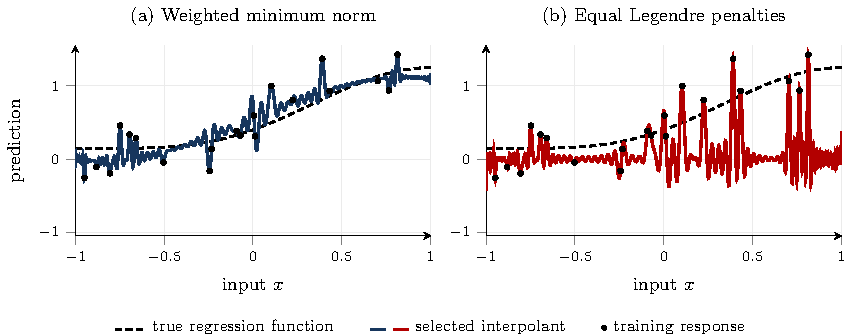
\includegraphics[width=\linewidth]{../figures/lecture09-polynomial-interpolants-plot.pdf}
\caption{Both panels use the same $n=20$ observations from
$X\sim\operatorname{Unif}[-1,1]$ and
$Y=f^\star(X)+\cN(0,0.28^2)$, where
$f^\star(x)=0.55+0.55\sin(\pi x/2)-0.15\cos(\pi x)$, and the same space of
dimension $164$. Both rules interpolate. The weighted norm distinguishes
the first $m=4$ features; equal Legendre penalties minimize $L^2(\mu)$ norm.}
\label{fig:polynomial-interpolants}
\end{figure}


\Needspace{6\baselineskip}
\Cref{fig:polynomial-interpolants} shows both outcomes on one sample. The
weighted minimum-norm rule follows the smooth nonpolynomial regression
function between the observations. Equal penalties on the Legendre
coefficients select a function that stays close to zero over most of the
domain and makes narrow excursions to the observed responses. Both rules use
the same polynomial space and interpolate the same data. The selection rule
changes the population behavior. This comparison directs attention from the
size of the available model to the procedure that selects one interpolant.
Later sections establish asymptotic versions of both outcomes.%
\endnote{Dimension in the illustration. The sample size is $n=20$, the signal
block has size $m=4$, and the interpolation block has size $D=8n=160$. A
generic feature space of total dimension at least $n$ can already permit exact
interpolation. The positive bound later contains an $n/D$ term and additional
conditioning requirements, so a larger interpolation block makes its
population cost smaller. The displayed value makes the finite-sample contrast
clear and is an illustrative choice. Smaller values of $D$ also interpolate
this sample, with a less pronounced separation. The asymptotic corollary uses
the sufficient schedule $D_n=n^3$.}
\endnote{Scope of the illustration. A neural-network curve would specify one
architecture, parameterization, optimizer, initialization, and stopping rule;
a Laplace-kernel curve would specify one bandwidth. A single curve would not
represent either family. The polynomial rules in the figure make the two
selection procedures exact, and the main text analyzes their population
behavior.}

We therefore study the following descriptive question:

\begin{quote}
For which fixed data-generating laws does a specified interpolating learning
procedure have vanishing population excess risk?
\end{quote}

To make the question precise, fix a nonempty measurable input space $\cX$, and let
$\cP_2$ be the class of probability laws $P$ on $\cX\times\R$ satisfying
$\E_P[Y^2]<\infty$. Let
$S_n=((X_1,Y_1),\ldots,(X_n,Y_n))$ be an i.i.d. sample from a fixed
$P\in\cP_2$. Write $\mu=P_X$ and
\[
 f_P^\star(x)=\E[Y\mid X=x].
\]
For functions, $\|f\|_2$ abbreviates $\|f\|_{L^2(\mu)}$ for the current
input law $\mu$.
For an independent test pair $(X,Y)$ with law $P$ and a fixed predictor
$f\in L^2(\mu)$, the squared-loss identity
\begin{equation}
 \E[(f(X)-Y)^2]-\E[(f_P^\star(X)-Y)^2]
 =\|f-f_P^\star\|_{L^2(\mu)}^2
 \label{eq:excess-l2}
\end{equation}
shows that learning the conditional mean is exactly the problem of making the
$L^2(\mu)$ error small. For a predictor selected from $S_n$, apply this identity
conditional on $S_n$. Its excess risk is then a random variable determined by
the training sample. \Cref{ex:l9-excess-risk-identity} asks you to prove both
claims.

\begin{definition}[Interpolating procedure and the benign set]
\label{def:benign-set}
Let $B=(B_n)_{n\ge1}$ be a fixed learning procedure, including any
predetermined choices of model dimension, feature scaling, norm, and
optimization rule. In a sample $S_n$, call index $i$ \emph{nonconflicting} if
$X_j=X_i$ implies $Y_j=Y_i$ for every $j$. For fixed $n$, call $B_n$
\emph{interpolating} if, for every sample,
\[
 B_n(S_n)(X_i)=Y_i,
 \qquad\text{for every nonconflicting index }i.
\]
Call $B$ interpolating if every $B_n$ is interpolating. For such a procedure,
define
\begin{equation}
 \cA(B)=\left\{P\in\cP_2:
 \|B_n(S_n)-f_P^\star\|_{L^2(P_X)}^2\xrightarrow{\P}0 \text{ as }n\to \infty
 \right\}.
 \label{eq:benign-set}
\end{equation}
For $P\in\cA(B)$, we say that the overfitting performed by $B$ on $P$ is
\emph{benign}.
\end{definition}

Repeated copies with the same response are nonconflicting; only a group that
assigns different responses to the same input is omitted. The definition
allows arbitrary input laws. Each optimization procedure below is understood
to impose constraints only at nonconflicting inputs.

On noisy problems, \emph{overfitting} refers here to exact fitting of realized
response noise. The word \emph{benign} refers to the vanishing population
excess risk. Thus interpolation names the fitting requirement, while
\emph{benign overfitting} names the combination. This is the standard term in
the recent literature.%
\endnote{Classification and regression. The random-label experiments of
\citet{zhang2017} brought the same question into the study of deep networks.
Let $\eta_k(x)$ be the clean conditional probability of class $k$. If a
training label is replaced by a uniformly random class with probability $p$,
then $\widetilde\eta_k(x)=(1-p)\eta_k(x)+p/K$. For $p<1$, the most likely class
is unchanged and every probability gap is multiplied by $1-p$. An
interpolating classifier fits the observed classes while the clean zero-one
target remains the Bayes class. In squared-loss regression, the interpolator
fits noisy responses while the population target remains the conditional
mean. Zero-one loss asks for the conditional mode; squared loss asks for the
conditional mean.}

How strong is it to prove that $\cA(B)$ is nonempty? By itself, this is a
vacuous requirement.

\begin{proposition}[Why nonemptiness alone is automatic]
\label{prop:automatic-nonempty}
Every interpolating procedure $B$ satisfies $\cA(B)\ne\varnothing$.
\end{proposition}

\begin{proof}
Fix $x_0$ and $y_0$, and let $P$ assign probability one to $(x_0,y_0)$.
Every sample consists only of copies of this pair. Interpolation forces
$B_n(S_n)(x_0)=y_0$, while $f_P^\star(x_0)=y_0$. Since the test input equals
$x_0$ almost surely, the population excess risk is zero for every $n$.
\end{proof}

The interpolation question is most informative when the responses contain
nondegenerate noise, meaning
\[
 \sigma_P^2:=\E[(Y-f_P^\star(X))^2]>0.
\]
If $Y=f_P^\star(X)$ almost surely, every observed response is a target value,
so exact fitting creates no direct conflict with estimating the target. A poor
selection rule can still fail between observations. With response noise,
interpolation additionally forces the procedure to fit random deviations from
the target. We therefore seek noisy members and nonmembers of benign sets.

\section{Interpolation is compatible with \texorpdfstring{$L^2$}{L2} approximation}
\label{sec:point-corrections}

Can interpolation preserve the accuracy of an estimator that already
generalizes? The setup asks for an interpolating procedure and vanishing
population error, but these properties concern different inputs: exact fitting
concerns the observations, while integrated loss concerns a fresh input. Start
with a consistent kernel smoother, or any other consistent regression
estimator, and modify its values only at the observations.

\begin{proposition}[Point-corrected smoother]
\label{prop:point-correction}
Suppose that $\mu(\{x\})=0$ for every $x\in\cX$, and that
$\widetilde f_n$ is any estimator
satisfying
\[
 \|\widetilde f_n-f_P^\star\|_{L^2(\mu)}\xrightarrow{\P}0
 \qquad\text{as }n\to\infty.
\]
For an arbitrary sample, let $I_n(S_n)$ contain one representative of every
distinct nonconflicting input, and define
\begin{equation}
 \widehat f_n(x)=\widetilde f_n(x)
 +\sum_{i\in I_n(S_n)}
   \bigl(Y_i-\widetilde f_n(X_i)\bigr)\I\{x=X_i\}.
 \label{eq:point-corrected}
\end{equation}
Then the resulting procedure is interpolating, and
\[
 \|\widehat f_n-f_P^\star\|_{L^2(\mu)}
 =\|\widetilde f_n-f_P^\star\|_{L^2(\mu)}
 \xrightarrow{\P}0
 \qquad\text{as }n\to\infty.
\]
\end{proposition}

\begin{proof}
For every sample, substituting a nonconflicting input into
\cref{eq:point-corrected} gives $\widehat f_n(X_i)=Y_i$. Thus the procedure is
interpolating. The assumption on $\mu$ makes every finite set have measure
zero. The difference
$\widehat f_n-\widetilde f_n$ is supported on the finite set
$\{X_1,\ldots,X_n\}$. Therefore its
$L^2(\mu)$ norm is zero. In particular, the triangle inequality gives
\begin{align*}
 \|\widehat f_n-f_P^\star\|_{L^2(\mu)}
 &\le \|\widetilde f_n-f_P^\star\|_{L^2(\mu)}
    +\|\widehat f_n-\widetilde f_n\|_{L^2(\mu)}\\
 &=\|\widetilde f_n-f_P^\star\|_{L^2(\mu)}.
\end{align*}
The reverse inequality holds because the two functions agree
$\mu$-almost everywhere.
\end{proof}

The added terms change only the observed point values.\endnote{Point
corrections. The functions $\I\{x=X_i\}$ are point indicators, sometimes
informally called ``spikes.''}\label{en:point-indicators}
The result proves that interpolation and
$L^2$ consistency can coexist. Its selection rule is an explicit point
correction; gradient training of a neural network uses a different rule.
In \cref{ex:l9-point-corrections}, you are asked to show that averaging the
responses observed at each distinct input extends the construction to
arbitrary input laws under the interpolation convention in
\cref{def:benign-set}.

Can the benign set equal the full problem class? Let
$\cC\subseteq\cP_2$ be a
class on which one fixed base procedure $\widetilde B$ is $L^2$-consistent.
Point correction produces one interpolating procedure $B$ with
$\cC\subseteq\cA(B)$ when the laws in $\cC$ have no point masses; response
averaging gives the same conclusion for arbitrary input laws. In particular,
a universally consistent base procedure yields an interpolating procedure
whose benign set is the full problem class on which universality holds.
Standard universally consistent regression procedures, with truncation for
unbounded responses, provide such bases on Euclidean input spaces.

Consequently, no negative theorem can show that every interpolating learning
procedure fails on some law in such a class. A negative result must restrict
the learning procedure, its output geometry, or the required mode of risk
control.

\section{A minimum-norm polynomial interpolator}
\label{sec:series}

Can a neural network trained by gradient descent to interpolation have a
nontrivial benign set $\cA(B)$? The predictor selected by gradient descent in
a finite nonlinear network is difficult to characterize. We therefore study
the corresponding linear problem, where the selected interpolant can be
described exactly.

In the linear setting, the link with gradient training is exact. In
Problem~3 of Homework~0, you were asked to prove that, for a full-row-rank
design matrix, gradient descent on the squared loss, started at zero with
a sufficiently small constant step size, converges to the interpolating
parameter vector of smallest Euclidean norm. Gradient flow started at zero
selects the same vector. The next lecture will develop this connection further.
Minimum-norm interpolation is
therefore the natural linear analogue of interpolation by gradient training.
Formally, let $\varphi: \cX \to \R^p$ be some fixed function, collecting
the $p\ge n$ basis functions to be used. A linear combination of the underlying
basis functions takes the form 
\[
f_\theta(x) = \theta^\top \varphi(x)\qquad (x\in \cX)\,.
\]
The minimum norm interpolant is then $f_{\hat\theta}$ where 
$\hat\theta$ solves the problem
\begin{align}
\min \|\theta\| \qquad \text{ subject to } \qquad \theta\in \R^p, \qquad
f_\theta(X_i)=Y_i,\quad 1\le i \le n\,.
\label{eq:minnorm}
\end{align}
Above, $\|\cdot\|$ is the $2$-norm, because this is what is selected for by
gradient descent.
The problem has a solution as long as the $n\times p$ matrix whose $(i,j)$th
element is $\varphi_j(X_i)$ has rank $n$. For now, assume this is the case.
The solution is unique whenever at least one solution exists.
\Cref{ex:l9-minimum-norm} asks you to prove uniqueness and derive the
minimum-norm solution.

While the norm above is fixed to the $2$-norm, 
by linearly combining the basis functions, one can change
what interpolant will be selected, while leaving the set
of functions that can be represented intact.
To see how this works let 
$G$ be an invertible $p\times p$ matrix and consider replacing $\varphi$ above with
$\varphi^{(G)}(x):=G\varphi(x)$. Correspondingly, let $f^{(G)}_c(x):= c^\top \varphi^{(G)}(x)$.
On the one hand, 
\[
\cF:=\{ f_\theta \,:\, \theta\in \R^p \} = \{ f^{(G)}_c\,:\, c\in \R^p \}\,,
\]
while for all $\theta\in \R^p$,
\[
f_\theta(x) = \theta^\top G^{-1} G \varphi(x) = (G^{-T}\theta)^\top \varphi^{(G)}(x) = f^{(G)}_{G^{-T}\theta}(x)\,.
\]
Hence, the norm $\|\theta\|$ becomes $\|G^{-T}\theta\|$ when changing
the basis functions from $\varphi$ to $\varphi^{(G)}$.

One can make this more explicit by introducing a norm on $\cF$ based on
choosing a set of basis functions that span $\cF$. In particular, for any 
$\psi: \cX \to \R^p$ such that $\cF = \{ x\mapsto \theta^\top \psi(x)\,:\, \theta\in \R^p \}$,
for $f\in \cF$, let 
\[
\|f\|_{\psi}:= \inf\{ \|\theta\| \,:\, f(\cdot) = \theta^\top \psi(\cdot)\,, \theta\in \R^p\}\,.
\]
One can then show that $\|\cdot\|_{\psi}$ is indeed a norm on $\cF$ (when $\cF$ is viewed as a vector space
over the reals with the usual operations).
Also, the optimization problem in \cref{eq:minnorm} is equivalent to 
\begin{align}
\min \|f\|_{\varphi} \qquad \text{ subject to } \qquad f\in \cF, \qquad
f(X_i)=Y_i,\quad 1\le i \le n\,
\label{eq:minnormsubspace}
\end{align}
in the sense that if $f^\star$ is a solution to this problem and $\theta^\star$ is a solution to
 \cref{eq:minnorm} then $f^\star = f_{\theta^\star}$.
Finally, with this notation it is clear that switching from $\varphi$ to $\varphi^{(G)}$
changes the optimization problem so that the norm
$\|f\|_{\varphi}$
in \cref{eq:minnormsubspace} is replaced
by 
$\|f\|_{\varphi^{(G)}}$.
\Cref{ex:l9-induced-function-norm} asks you to verify these claims, including
the case of linearly dependent features.

\subsection{Benign overfitting with polynomials}
In the rest of this section we consider the case when an unknown regression function
is to be approximated by polynomials with the goal of demonstrating 
how one can achieve benign overfitting for a reasonably large problem class.
In particular, we will consider polynomial approximation of smooth functions.
For simplicity, we consider the case when $\cX = [-1,1]$ and when $\mu = P_X$ is uniform on this domain.
Retain the i.i.d. sampling setup above, write $f^\star=f_P^\star\in L^2(\mu)$,
and assume that, for some $\sigma^2<\infty$,
\begin{equation}
 Y_i=f^\star(X_i)+\varepsilon_i,\qquad
 \E[\varepsilon_i\mid X_i]=0,\qquad
 \E[\varepsilon_i^2\mid X_i]\le\sigma^2.
 \label{eq:legendre-model}
\end{equation}
The conditional variance may depend on the input.

For $g:\R\to\R$, recall that $g$ is a polynomial of degree $r$ ($\deg(g)=r$)
if for every $x\in \R$, $g(x) = \sum_{i=0}^r a_i x^i$ with some coefficients $(a_i)_i$ with $a_r\ne 0$.
Set $\deg(0)=-\infty$ so that the zero polynomial is included below.
Let $\cF_r$ denote the set of polynomials of degree below $r$:
$\cF_r = \{ g \,:\, g \text{ is a polynomial and } \deg(g)<r \}$. Note that this is
an $r$-dimensional subspace of $\R^{\R}$ (and by restricting the functions to $\cX$ of $\R^\cX$).
Given $f^\star\in L^2(\mu)$,
define the best
squared approximation error of approximating $f^\star$
with polynomials of degree below $m$ to be
\begin{equation}
 A_m(f^\star)=\inf_{g\in \cF_m}\|g-f^\star\|_{L^2(\mu)}^2\,.
 \label{eq:approximation-error}
\end{equation}
For $s>0$, say that $f^\star$ has
\emph{polynomial approximation order $s$} if, for some fixed $L<\infty$,
\begin{equation}
 A_m(f^\star)\le L^2m^{-2s},\qquad m\ge1.
 \label{eq:s-smooth-approximation}
\end{equation}
Jackson approximation estimates imply this condition for the usual
$s$-smooth classes. For example, for integer $s\ge1$, membership in the
Sobolev space $W^{s,2}([-1,1])$ suffices: $f^\star$ and its weak derivatives
through order $s$ are square integrable. Lipschitz functions satisfy the
condition with $s=1$.
Classical regression bounds balance squared approximation error of order
$m^{-2s}$ with estimation error of order $m/n$, giving the squared
$L^2(\mu)$ error rate $n^{-2s/(2s+1)}$. Achieving this balance by polynomial
least squares also requires control of the sampled design matrix. Under
uniform sampling, the sufficient condition used below is
$m^2\log m=o(n)$; the balancing choice $m\asymp n^{1/(2s+1)}$ satisfies it
when $s>1/2$. The exponent is minimax optimal over bounded $s$-smooth
classes under standard nondegenerate noise assumptions. No estimator
achieves a faster rate uniformly over such a class.
The bibliographical notes give references for approximation,
least-squares stability, and minimax optimality separately.

The challenge we consider is whether the same rate can be obtained by using minimum-norm
interpolants -- even when the responses are noisy. 
This is a challenge because normal least-squares fitting does not interpolate.
Indeed, the best polynomial (as defined in \cref{eq:approximation-error}) approximator,
given any degree $r$, 
only depends on the $f^\star$, hence, this polynomial will \emph{not} interpolate.
Also, standard least-squares fitting, would not interpolate. In fact it is considered
a strength of least-squares fitting that it ``cleans'' (or ``smoothens''), 
separating signal ($f^\star$) from noise.

It also follows that to meet the challenge we need to make a deliberate choice of what coordinate (basis)
functions we use to parametrize the chosen subspace $\cF_p$. First, as noted beforehand,
$p\ge n$ is necessary for allowing for interpolation. 
Our strategy will be to split $p=m+D$ into
$m\ll p$ basis functions that will span $\cF_m$ -- the goal of these is to capture
the signal in the data --, and a remaining set of extra $D$ basis functions, whose purpose 
will be to fit to the noise.
In particular, we choose the basis and scaling of these two blocks so that the selected
interpolant represents the low-degree component in the first block and uses
the second block for sample-specific residuals with small population $L^2$
norm,
essentially 
following the strategy used by the point-corrected smoother of \cref{prop:point-correction}.

For the first block, let $P_j$ be the degree-$j$ Legendre polynomial
normalized by $P_j(1)=1$, and set
\[
 \psi_j(x)=\sqrt{2j+1}\,P_j(x),\qquad j\ge0.
\]
The functions $(\psi_j)_{j\ge0}$ form an orthonormal basis of $L^2(\mu)$.
\Cref{app:l2-background} reviews $L^2$ spaces, inner products, Hilbert
spaces, and orthonormal bases.
The significance of this choice is that 
for any $\beta = (\beta_j)_j$, $m\ge 1$,
$\|\sum_{j=0}^{m-1} \beta_j \psi_j\|_{L^2(\mu)}^2 = \sum_{j=0}^{m-1} \beta_j^2 = \|\beta\|^2$.
Minimizing the coefficient $2$-norm is the same as minimizing the $L^2(\mu)$ norm of the underlying function.

For the second block, define
\[
 \chi_0(x)=1,\qquad
 \chi_j(x)=\sqrt2\,T_j(x)\quad(j\ge1),\qquad
 T_j(\cos\theta)=\cos(j\theta).
\]
The functions $\chi_j$ are uniformly bounded by $\sqrt2$ and orthonormal
under the arcsine law $\nu(dx)=dx/(\pi\sqrt{1-x^2})$. Since
$\mu\le(\pi/2)\nu$ (in the sense that $\mu(A)\le (\pi/2)\nu(A)$ for any $A\subset \R$ Borel),
\begin{equation}
 \left\|\sum_jb_j\chi_j\right\|_{L^2(\mu)}^2
 \le\frac\pi2\sum_jb_j^2
 \label{eq:chebyshev-synthesis}
\end{equation}
for every finite coefficient vector. \Cref{ex:l9-orthogonal-projection}
asks you to justify both this inequality and the orthonormal norm identity.
Thus the first block has exact
population-norm accounting, while the second has the upper bound needed to
control the population cost of interpolation.

Combining the two blocks gives the feature map
\begin{equation}
 \phi_{m,D}(x)=
 \bigl(\psi_0(x),\ldots,\psi_{m-1}(x),
 D^{-1/2}\chi_m(x),\ldots,D^{-1/2}\chi_{m+D-1}(x)\bigr)^\top.
 \label{eq:scaled-feature-map}
\end{equation}
The factor $D^{-1/2}$ is the central design choice. The $D$ additional
features can collectively fit an arbitrary residual vector. On the sample
event established below, the unscaled features can fit a residual $z$ with
coefficient squared norm at most $C\|z\|^2/D$. Without rescaling, increasing
$D$ would therefore make it progressively cheaper in parameter norm to fit
the entire response with the additional block. Multiplication by
$D^{-1/2}$ multiplies this parameter cost by $D$. A fixed low-degree
component then has bounded cost in the first block and reduces the residual
cost across all $n$ observations; the sample-specific remainder is fitted by
the second block. Its population squared norm remains at most
$C\|z\|^2/D$.

Write a predictor in these coordinates as
\[
 f_{\beta,b}(x)=\sum_{j<m}\beta_j\psi_j(x)
             +\sum_{j=m}^{m+D-1}b_j\chi_j(x),
 \qquad \theta=(\beta,\sqrt D\,b).
\]
Then $f_{\beta,b}(x)=\theta^\top\phi_{m,D}(x)$ and
\begin{equation}
 \|\theta\|^2=\|\beta\|^2+D\|b\|^2.
 \label{eq:weighted-series-norm}
\end{equation}
The factor $D$ in this expression is therefore induced by the feature
scaling. The empirical-loss objective remains unregularized, and the
procedure minimizes this parameter norm subject to exact interpolation.

The combined features have successive polynomial degrees and nonzero leading
coefficients, so they span all polynomials of degree less than $m+D$. At $n$
distinct inputs their evaluation matrix has row rank $n$, provided $m+D\ge n$.
The procedure
therefore interpolates arbitrary responses almost surely. The remaining
question is whether its population error vanishes.

\subsection{Approximation, estimation, and interpolation cost}

How accurately does this optimization procedure estimate $f^\star$?
We use the low-degree component to estimate a polynomial approximation and
show that the extra component has small population norm:

\Needspace{12\baselineskip}
\begin{theorem}[Benign overfitting for weighted polynomial interpolation]
\label{thm:weighted-legendre}
Under the uniform-input model \cref{eq:legendre-model}, there are universal
constants $c,C>0$ such that, if $m+D\ge n$ and $D\ge16m$, then for
every $\delta\in(0,1)$, with probability at least
\[
 1-Cn^2/D-m\exp(-cn/m^2)-\delta,
\]
the weighted minimum-norm interpolator $\widehat f$ satisfies
\begin{align}
 \|\widehat f-f^\star\|_{L^2(\mu)}^2
 \le\frac C\delta\bigg(&A_m(f^\star)+\frac{\sigma^2m}{n}
       +\frac{\|f^\star\|_{L^2(\mu)}^2}{n^2}
       +\frac nD\bigl(\|f^\star\|_{L^2(\mu)}^2+\sigma^2\bigr)\bigg).
 \label{eq:legendre-bound}
\end{align}
\end{theorem}

There are a number of observations to be made about this result.
First, to control the error probability, it is not enough to choose $\delta$ small
and $n$ large. One also needs to choose $D$ to be large relative to $n^2$.
Second, the dependence of the error bound on $\delta$ may look unexpectedly
weak. This is the result of deliberately loose analysis: The present bound will be sufficient
for our purposes (see \cref{cor:s-smooth-consistency}) and the analysis can be shorter
this way. The third observation is that the error bound in \cref{eq:legendre-bound} has
familiar and less familiar terms. 
In particular, the first two terms are familiar from
standard analysis of regression: the approximation and estimation errors need to be 
balanced to get good outcomes. If we used $m$ coefficients with standard 
linear least squares, these are the terms one would expect to see.
The next, third term, is a small shrinkage bias.
The last term is unusual: This is the price of fitting to the residual error
(after the first $m$ coefficients are used to get the ``signal''). To make this 
error small, $D$ needs to be chosen large relative to $n$ (similarly to how
$D$ needs to be large to control the error probability).
For a fixed $n$, to get the best possible error bound,
first one could choose a value of $m$ to balance between the first
two terms (while also paying attention to the error probability term), 
after which the value of $D$ is dictated by the need to control
the last term (and the error probability term).
Increasing $D$ supplies more directions over which to
distribute the interpolation correction. 
Surprisingly, increasing $D$ has no price attached to it -- other than
the increased computation and memory costs. 
This is because of the careful selection of the weighting of the Chebyshev polynomial
basis functions: As $D$ gets large, these are appropriately downweighted 
and as such, the upper bound on the squared error of the resulting residual component decreases as $D$ increases.
In effect, the procedure closely follows what the point-correction mechanism is aimed
to achieve: The function that is learnt with the last $D$ coefficients approximates
the point-mass correction, while the function that is learnt with the first $m$ 
coefficients approximates the function that would be learnt using just those basis functions.

Again, the intuitive explanation is that when solving for the minimum norm interpolant,
the price for the last $D$ coefficients is much higher than for the first $m$. 
The result of this is essentially a two-step fitting: First fit using the first $m$
coefficients, then use the last $D$ coefficients to approximate the residual.
\Cref{ex:l9-two-stage-fitting} asks you to make this comparison precise
and bound the difference between the coefficient vectors. In general,
the first stage is generalized least squares, with residual weight
$(VV^\top)^{-1}$ for the second block's sample matrix $V$, defined next.
It reduces to ordinary least squares when $VV^\top$ is a scalar multiple
of $I_n$.

Define
\[
 U_{ij}=\psi_j(X_i)\ (0\le j<m),\qquad
 V_{ij}=\chi_{m+j}(X_i)\ (0\le j<D),\qquad
 H=D^{-1}VV^\top.
\]
Let $u=(\psi_0,\ldots,\psi_{m-1})^\top$ and
$v=(\chi_m,\ldots,\chi_{m+D-1})^\top$.
For matrices, $\|\cdot\|$ denotes the Euclidean operator norm, and
$S\preceq R$ means that $R-S$ is positive semidefinite.
In 
\cref{app:legendre-proof}, it is shown that
for universal constants $c_H,C_H,c_{\rm pr},C_{\rm pr}>0$, there is an
event $\cG$ determined by the inputs such that
\begin{equation}
 c_HI_n\preceq H\preceq C_HI_n,
 \qquad U^\top U\succeq(n/2)I_m
 \qquad \text{while}
 \qquad \P(\cG^c)\le C_{\rm pr}n^2/D
       +m\exp(-c_{\rm pr}n/m^2).
 \label{eq:good-event-summary}
\end{equation}
The second condition makes the low-degree coefficients estimable. To see
the role of the first, fix any vector $z\in\R^n$, meant to model the ``residual errors'' after
removing the ``signal''. 
On $\cG$, the
coefficients $b_z=V^\top(VV^\top)^{-1}z$ give $Vb_z=z$, while
\begin{equation}
 \|b_z^\top v\|_{L^2(\mu)}^2
 \le\frac\pi2\|b_z\|^2
 =\frac\pi2 z^\top(VV^\top)^{-1}z
 \le\frac{\pi}{2c_HD}\|z\|^2.
 \label{eq:residual-interpolation-cost}
\end{equation}
The first inequality is due to \cref{eq:chebyshev-synthesis}, while the last is 
from $VV^\top=DH\succeq c_HD I_n$.
A residual vector with squared length of order $n$ can therefore be fitted
at population cost of order $n/D$. This is the interpolation mechanism. It
uses a population-norm bound for the second block and a well-conditioned
sample Gram matrix.

\begin{proof}[Proof of \cref{thm:weighted-legendre}]
Let $\cG$ be the input event supplied by \cref{eq:good-event-summary}.
As noted above, \cref{app:legendre-proof} proves
\cref{eq:good-event-summary}. Let $\Delta:=\|\widehat f-f^\star\|_{L^2(\mu)}^2$.
Now, for any $s\ge 0$,
\[
\P( \Delta>s ) \le \P( \Delta>s, \cG) + \P( \cG^c) = 
\P( \one{\cG}\Delta>s) + \P( \cG^c)\,,
\]
where the last equality holds because 
$\{\Delta>s\}\cap \cG = \{\one{\cG}\Delta>s\}$. 
Indeed,
if $\cG$ holds and $\Delta>s$, $\one{\cG}=1$ and thus $\one{\cG}\Delta>s$ also holds
and if $\one{\cG}\Delta>s$ then $\one{\cG}=1$ must be true (since $s$ is nonnegative),
hence $\cG$ holds and also $\Delta>s$ holds. 
Now, choosing 
$s = \tfrac{1}{\delta}\,\E[\one{\cG}\Delta]$,
from Markov's inequality we get
\[
\P\left( \Delta > \tfrac{1}{\delta}\,\E[\one{\cG}\Delta]\right) \le \delta+\P(\cG^c)\,.
\]
If $\E[\one{\cG}\Delta]=0$, the same conclusion follows because
$\one{\cG}\Delta=0$ almost surely. Hence, it suffices to bound
$\E[\one{\cG}\Delta]$ by $C$ times the expression in parentheses in
\cref{eq:legendre-bound}.

Define the two
coefficient vectors together by
\[
 (\widehat\beta,\widehat b)
 =\arg\min_{\beta\in\R^m,\,b\in\R^D}
 \left\{\|\beta\|^2+D\|b\|^2:
 \mathbf Y=U\beta+Vb\right\}.
\]
Let
\[
 g_m=\beta_\star^\top u
 =\arg\min_{g\in\cF_m}\|g-f^\star\|_{L^2(\mu)}^2
\]
be the best degree-$(m-1)$ polynomial approximation of $f^\star$ in
$L^2(\mu)$, and put $r=f^\star-g_m$. Then
\begin{align}
 \|r\|_{L^2(\mu)}^2=A_m(f^\star),\qquad
 \|\beta_\star\|^2=\|g_m\|_{L^2(\mu)}^2
 \le
 \|g_m\|_{L^2(\mu)}^2+\|r\|_{L^2(\mu)}^2=
 \|f^\star\|_{L^2(\mu)}^2. \label{eq:betastarbound}
\end{align}
Here, $\|\beta_\star\|^2=\|g_m\|_{L^2(\mu)}^2$ is due to the choice of the orthonormal basis $u$, and the last equality
is because the optimality of $g_m$ makes $r$ orthogonal to $g_m$.
\Cref{ex:l9-orthogonal-projection} asks you to prove this orthogonality
and the resulting Pythagorean identity.

Set $h=\widehat b^\top v$. Since
\[
 \widehat f-f^\star
 =(\widehat\beta-\beta_\star)^\top u+h-r
\]
from the triangle inequality, $(a+b+c)^2 \le 3(a^2+b^2+c^2)$, 
and because the components of $u$ are orthonormal in $L^2(\mu)$, we get
\begin{equation}
 \Delta=\|\widehat f-f^\star\|_{L^2(\mu)}^2
 \le3\|\widehat\beta-\beta_\star\|^2
    +3\|h\|_{L^2(\mu)}^2+3A_m(f^\star).
 \label{eq:three-errors}
\end{equation}
(Since the feature groups are not orthogonal in $L^2(\mu)$, the triangle inequality is the best tool we have.)

It remains to bound $\E[ \one{\cG}\|\widehat\beta-\beta_\star\|^2]$ and $\E[\one{\cG}\|h\|_{L^2(\mu)}^2]$.
To bound these, the next step is to calculate $(\widehat \beta,\widehat b)$ in closed form.
For this, we first separate the minimization over the two
coefficient blocks:
\begin{align*}
\MoveEqLeft
\min\{\|\beta\|^2+D\|b\|^2:
       \mathbf Y=U\beta+Vb,\ \beta\in\R^m,\ b\in\R^D\}\\
&=\min\left\{
   \min\{\|\beta\|^2+D\|b\|^2:
          \mathbf Y=U\beta+Vb,\ b\in\R^D\}:
   \beta\in\R^m\right\}\\
&=\min\left\{
   \|\beta\|^2+
   \min\{D\|b\|^2:
          \mathbf Y=U\beta+Vb,\ b\in\R^D\}:
   \beta\in\R^m\right\}.
\end{align*}
For fixed $\beta$, the minimum-Euclidean-norm solution of
$Vb=\mathbf Y-U\beta$ on $\cG$ is
\begin{align}
 b_\beta=V^\top(VV^\top)^{-1}(\mathbf Y-U\beta).  
 \label{eq:bbeta}
\end{align}
By algebra, we get
$ D\|b_\beta\|^2
 =(\mathbf Y-U\beta)^\top H^{-1}(\mathbf Y-U\beta)$.
Plugging this value into the outer problem reduces it to minimizing
$\|\beta\|^2
 +(\mathbf Y-U\beta)^\top H^{-1}(\mathbf Y-U\beta)$.
Setting the derivative of this with respect to $\beta$ to zero and solving gives
\begin{equation}
 \widehat\beta=(I_m+U^\top H^{-1}U)^{-1}
 U^\top H^{-1}\mathbf Y.
 \label{eq:beta-hat}
\end{equation}
\Cref{ex:l9-minimum-norm} asks you to supply the linear algebra and
differentiation steps in this elimination.

Write $r_X=(r(X_i))_{i=1}^n$. Then, 
from $f^\star = g_m + f^\star-g_m = \beta_\star^\top u + r$
and $Y_i = f^\star(X_i)+\varepsilon_i$
we get
\begin{align}
  \mathbf Y=U\beta_\star+r_X+\boldsymbol\varepsilon\,.
  \label{eq:datarx}
\end{align}
On $\cG$, define
\[
 A=U^\top H^{-1}U,
 \qquad T=(I_m+A)^{-1}U^\top H^{-1}\,,
\]
and set $A=0$ and $T=0$ on $\cG^c$ when taking expectations below. On $\cG$,
\cref{eq:beta-hat}
 becomes $\widehat \beta = T \mathbf Y$, which combined with  \cref{eq:datarx}
 gives
\begin{equation}
 \widehat\beta-\beta_\star
 =-(I_m+A)^{-1}\beta_\star+Tr_X+T\boldsymbol\varepsilon\,,
 \label{eq:beta-error}
\end{equation}
thus,
\begin{align*}
\|\widehat\beta-\beta_\star\|^2
& \le 
 3( \|(I_m+A)^{-1}\|^2 \, \| \beta_\star\|^2+\|Tr_X\|^2+\|T\boldsymbol\varepsilon\|^2)\\
&\le
 3( \|(I_m+A)^{-1}\|^2 \, \| f^*\|_{L^2(\mu)}^2+\|T r_X\|^2+\|T \boldsymbol\varepsilon\|^2)\,,
\end{align*}
where the last inequality used that by
\cref{eq:betastarbound}, $\| \beta_\star\|^2\le \| f^*\|_{L^2(\mu)}^2$.

Since we need to bound $\E[ \one{\cG}\|\widehat\beta-\beta_\star\|^2 ]$,
we turn to bounding the expectation of the three terms multiplied by the indicator of $\cG$.

We have $\|T r_X \|^2 =  r_X^\top T^\top T r_X \le \|T^\top T\|\, \|r_X \|^2$.
Thus, if $B_T$ is a deterministic upper bound on $\|T^\top T\|$ on $\cG$,
\[
\E[ \one{\cG} \|T r_X \|^2] \le B_T \,\E[ \|r_X\|^2]=B_T \,n\, \E[r^2(X_1)]
= B_T \,n\, \|r\|_{L^2(\mu)}^2
 =B_T\,n\,A_m(f^\star)\,.
\]

 \newcommand{\beps}{\boldsymbol\varepsilon}
 Next, defining $X_{1:n} = (X_1,\dots,X_n)$,
 we calculate $\| T \boldsymbol\varepsilon\|^2 =  \beps^\top T^\top T \beps = \trace(
   T^\top T \beps \beps^\top )$.
Thus, $\E[ \| T \boldsymbol\varepsilon\|^2\, | \,X_{1:n}] = \trace(T^\top T \E[\beps \beps^\top\,|\,X_{1:n} ]  )
\le \sigma^2 \,\trace(T^\top T I_n)
=\sigma^2\, \trace(T^\top T)
$, where the i.i.d. sampling assumption and \cref{eq:legendre-model} give
$\E[\beps\mid X_{1:n}]=0$ and
$\E[\beps\beps^\top\mid X_{1:n}]\preceq\sigma^2 I_n$.
Thus, 
\begin{align*}
 \E[ \one{\cG} \| T \boldsymbol\varepsilon\|^2 ]
 = 
\E\left[\,\E[ \one{\cG}\, \| T \boldsymbol\varepsilon\|^2 \,|\, X_{1:n} ]\,\right]
 \le
 \sigma^2\, \E[ \, \one{\cG} \trace(T T^\top) ]\,.
\end{align*}

Thus, it remains to bound $T T^\top$ and 
 $\|(I_m+A)^{-1}\|$ on $\cG$.
On $\cG$, the two sides of the bound on $H$ in
\cref{eq:good-event-summary} give
\[
 H^{-1}\succeq C_H^{-1}I_n,
 \qquad H^{-2}\preceq c_H^{-1}H^{-1}.
\]
Together with $U^\top U\succeq(n/2)I_m$, the first inequality yields
\[
 A=U^\top H^{-1}U\succeq C_H^{-1}U^\top U
 \succeq\frac{n}{2C_H}I_m.
\]
Hence
\begin{equation}
\begin{split}  
 \|(I_m+A)^{-1}\|
 &\le \frac{1}{1+n/(2C_H)}\le\frac{2C_H}{n},\\
 TT^\top
 &\preceq c_H^{-1}(I_m+A)^{-1}A(I_m+A)^{-1}
 \preceq\frac{2C_H}{c_Hn}I_m.
\end{split}
 \label{eq:T-bounds}
\end{equation}
From the last inequality and $\|T^\top T\|=\|TT^\top\|$, we see that we can choose
$B_T = \frac{2C_H}{c_Hn}$,
and we also have $\trace(T T^\top)\le \frac{2C_H m}{c_Hn}$.
\Cref{ex:l9-matrix-order,ex:l9-quadratic-forms} ask you to justify these
matrix-order, norm, and trace steps, including the conditional noise calculation.
Putting things together, we get 
\begin{equation}
 \E[\I\{\cG\}\|\widehat\beta-\beta_\star\|^2]
 \le C\left(\frac{\|f^\star\|_{L^2(\mu)}^2}{n^2}
            +A_m(f^\star)+\frac{\sigma^2m}{n}\right)
 \label{eq:head-risk}
\end{equation}
for some universal constant $C>0$.

We now turn to bounding $\|h\|_{L^2(\mu)}^2 = \| \widehat b^\top v \|_{L^2(\mu)}^2$ in
 \cref{eq:three-errors}.
By  \cref{eq:chebyshev-synthesis}, 
$\| \widehat b^\top v \|_{L^2(\mu)}^2 \le \frac\pi2\|\widehat b\|^2$, so it remains
to bound $\|\widehat b\|^2$.
For this, set
\[
K=UU^\top+H,\qquad \alpha=K^{-1}\mathbf Y.
\]
\Cref{ex:l9-push-through} asks you to derive the following identities from
the optimality equations and to verify them directly from
\cref{eq:bbeta,eq:beta-hat} using the push-through identity:
\[
 \widehat\beta=U^\top\alpha,
 \qquad \widehat b=D^{-1}V^\top\alpha.
\]
Thus $VV^\top=DH$ and $c_HI_n\preceq H\preceq K$ give
\begin{align}
\|\widehat b\|^2
 =\frac{1}{D}\alpha^\top H\alpha
 \le\frac{1}{D}\mathbf Y^\top K^{-1}\mathbf Y
 \le\frac{1}{c_HD}\|\mathbf Y\|^2.
 \label{eq:tail-cost}
\end{align}
Since
$
 \E[\|\mathbf Y\|^2]
 =n\E[Y_1^2]
 \le n(\|f^\star\|_{L^2(\mu)}^2+\sigma^2)$,
it follows that
\[
 \E[\I\{\cG\}\|h\|_{L^2(\mu)}^2]
 \le\frac{\pi n}{2c_HD}
       (\|f^\star\|_{L^2(\mu)}^2+\sigma^2).
\]
Combining this bound with \cref{eq:three-errors,eq:head-risk} gives the
required bound on $\E[\one{\cG}\Delta]$. The initial Markov argument and
the bound on $\P(\cG^c)$ then prove the theorem, after increasing $C$ to
cover both the risk bound and $C_{\rm pr}$, and taking $c=c_{\rm pr}$.
\end{proof}

\paragraph{Why use Chebyshev polynomials in the second block?}
The proof uses their population-norm bound
\cref{eq:chebyshev-synthesis} and the bounds on $H$ in
\cref{eq:good-event-summary}. Legendre polynomials would also give the
population-norm bound, with equality. The advantage of Chebyshev
polynomials is in controlling $H$ uniformly in the block of size $D$.
The boundedness and cosine representation of these polynomials imply that
\[
 H_{ii}=\frac1D\sum_{j=m}^{m+D-1}\chi_j(X_i)^2
\]
is bounded above and away from zero by universal constants when
$D\ge16m$. Their orthonormality under $\nu$, together with
$\mu\le(\pi/2)\nu$, also bounds the off-diagonal second moments:
$\E[H_{i\ell}^2]\le \pi^2/(4D)$ for $i\ne\ell$.
In \cref{app:legendre-proof}, these facts give both of the 
high probability
spectral bounds on
$H$. % except on an event of probability at most $C_{\rm pr}n^2/D$.
The upper bound on $H$ controls the estimation error through
$A=U^\top H^{-1}U$; the lower bound controls the coefficient cost of
fitting the residual in \cref{eq:tail-cost}.

For comparison, using the normalized Legendre polynomials in the second
block would give, at $x=1$,
\[
 \frac1D\sum_{j=m}^{m+D-1}\psi_j(1)^2
 =\frac1D\sum_{j=m}^{m+D-1}(2j+1)=2m+D.
\]
Thus the uniform diagonal upper bound used in this argument would fail.
Chebyshev polynomials supply that bound while retaining the
population-norm control needed for the interpolation component.
This is not merely a limitation of the proof: replacing the Chebyshev block
by Legendre polynomials while retaining the same scaling can destroy
consistency even for a bounded continuous target without observation
noise. In fact, \cref{thm:all-legendre-tuning} below establishes failure of
universal consistency for every deterministic choice of the two block
sizes.\endnote{\hypertarget{note:all-legendre-failure}{}An
all-Legendre variant can fail consistency. Replace only the second-block
functions $\chi_j$ by $\psi_j$, retaining the scaling in
\cref{eq:scaled-feature-map}. For a fixed sample of distinct interior inputs
and fixed $m$, as $D\to\infty$ the objective obtained by eliminating $b$
converges to
\[
 \|\beta\|^2+\frac\pi2\sum_{i=1}^n
 \sqrt{1-X_i^2}\bigl(Y_i-u(X_i)^\top\beta\bigr)^2.
\]
This is an unconstrained objective in $\beta$: the eliminated second block
still supplies the correction needed to interpolate. Its residual weights
are small near the endpoints. To see the consequence, define the weighted
population projection
\[
 Q_m f=\mathop{\rm argmin}_{g\in\cF_m}
 \int_{-1}^1\sqrt{1-x^2}\,|g(x)-f(x)|^2\,\mu(dx).
\]
With $m_n=\lfloor n^{1/4}\rfloor$, $D_n=n^3$, and noiseless responses
$Y_i=f^\star(X_i)$ for bounded $f^\star$, the all-Legendre interpolator
$\widehat f_n^{\rm Leg}$ satisfies
\[
 \|\widehat f_n^{\rm Leg}-Q_{m_n}f^\star\|_{L^2(\mu)}
 \xrightarrow{\P}0.
\]
This comparison uses Legendre kernel estimates and concentration of the
weighted design; the fixed-sample limit alone would not justify it.
However, $Q_m f^\star$ need not converge in the unweighted norm. An explicit
bounded continuous example is
\[
 N_k=2^{k^6},\qquad
 f^\star(x)=\sum_{k=1}^\infty\frac{\sin(N_k\arccos x)}{k^2}.
\]
The series converges uniformly, and $f^\star(-1)=f^\star(1)=0$.
Indeed, the polynomials $q_r(\cos\theta)=\sin(r\theta)/\sin\theta$
are orthogonal for the weighted projection, while
$\|q_r\|_{L^2(\mu)}^2=\sum_{j=1}^r(2j-1)^{-1}\sim\tfrac12\log r$.
The coefficient of $q_{N_k}$ in this example is asymptotic to
$2/(\pi k^2)$, so
\[
 \|Q_{N_k}f^\star-Q_{N_k-1}f^\star\|_{L^2(\mu)}\asymp k.
\]
At least one of the two projection errors therefore diverges along a
subsequence. Every integer $m$ occurs as $m_n$ (take $n=m^4$), so the
finite-sample comparison gives failure of consistency for the interpolator.
The difficulty concerns neighborhoods of the endpoints; changing values
at the two endpoints cannot change an $L^2(\mu)$ error.
}\label{en:all-legendre-failure}

\subsection{Consistency and rates}

Does the construction give a genuinely nontrivial benign set? 
As it turns out for our method the benign set cannot be further from being trivial:

\begin{corollary}[Universal consistency]
\label{cor:polynomial-benign-class}
Let $B^{\rm poly}$ use the feature map in
\cref{eq:scaled-feature-map} with
\[
 m_n=\max\{1,\lfloor n^{1/4}\rfloor\},\qquad D_n=n^3,
\]
and select the minimum-Euclidean-norm interpolant. With these choices, every law satisfying
\cref{eq:legendre-model} with $f^\star\in L^2(\mu)$ belongs to
$\cA(B^{\rm poly})$.
\end{corollary}
We call this a universal consistency result. ``Universal'' here refers to that 
the only restriction on the regression function $f^\star$ is that it needs to be 
square integrable with respect to $\mu$ (which is necessary anyways for the risk to be well-defined).
The law otherwise is a bit more restricted than what one usually sees in standard ``universal consistency''
results in that the we assumed a uniform bound on the noise variance. We note in passing that
with extra work, the results extend to the case when only the existence of the expected
risk is assumed.
In particular, \Cref{ex:l9-finite-variance} asks you to prove this extension.
The uniform conditional variance bound was responsible for the explicit
$\sigma^2m/n$ term; the exercise asks you to replace that term by a bound
depending on the tail of the conditional variance.

\begin{proof}
Polynomials are dense in $L^2(\mu)$, so
$A_{m_n}(f^\star)\to0$. Fix $\eta>0$ and apply
\cref{thm:weighted-legendre} with $\delta=\eta/2$. Every term on the
right-hand side of \cref{eq:legendre-bound} tends to zero, and the remaining
exceptional-event probability tends to zero. Hence
$\|B_n^{\rm poly}(S_n)-f^\star\|_{L^2(\mu)}^2\xrightarrow{\P}0$ as
$n\to\infty$.
\end{proof}

What rate is available when the target has additional structure? 
The target
enters the bound through $A_m(f^\star)$, while $m/n$ is the cost of estimating
the first $m$ coefficients from noisy observations.
Recall the polynomial approximation condition
\cref{eq:s-smooth-approximation} and the smoothness examples given there.
We next use these to derive that the minimum-norm interpolant is not only 
universally consistent, but also enjoys the best possible nonparametric
rates for smooth functions.

To state this result we recall the definition of the $O_{\P}(\cdot)$ notation:
For real random variables $Z_n$ and deterministic numbers $a_n>0$, the
notation $Z_n=O_{\P}(a_n)$ means that $Z_n/a_n$ is \emph{bounded in
probability}: for every $\delta>0$, there are a constant
$0<C_\delta<\infty$ and an integer $n_\delta$ such that
\[
 \P(|Z_n|>C_\delta a_n)\le\delta
 \qquad\text{for all }n\ge n_\delta.
\]
If $a_n\to0$, this implies $Z_n\xrightarrow{\P}0$. (However, note that no bound
on $\E[|Z_n|]$ follows from this.)

\begin{corollary}[$s$-smooth targets]
\label{cor:s-smooth-consistency}
Fix $s>1/2$ and choose
\[
 m_n=\max\{1,\lfloor n^{1/(2s+1)}\rfloor\},\qquad D_n=n^3.
\]
For every fixed target satisfying \cref{eq:s-smooth-approximation} and noise
law satisfying \cref{eq:legendre-model},
\begin{equation}
 \|\widehat f_n-f^\star\|_{L^2(\mu)}^2
 =O_{\P}\bigl(n^{-2s/(2s+1)}\bigr)\longrightarrow0
 \qquad\text{as }n\to\infty.
 \label{eq:s-smooth-rate}
\end{equation}
Thus these noisy problems belong to $\cA(B_s)$ for one predetermined
procedure $B_s$. For Lipschitz targets the rate is $O_{\P}(n^{-2/3})$.
\end{corollary}

\begin{proof}
The choices balance $A_{m_n}(f^\star)=O(m_n^{-2s})$ with $m_n/n$ at
order $n^{-2s/(2s+1)}$. The shrinkage and interpolation terms are $O(n^{-2})$.
Also $D_n\ge16m_n$ eventually,
$n/m_n^2\asymp n^{(2s-1)/(2s+1)}$ grows polynomially, and
$n^2/D_n=n^{-1}$. For any fixed error probability, choose $\delta$ smaller
than that probability. The other exceptional-event terms tend to zero,
giving the asserted bound in probability.
\end{proof}

Choosing $m_n$ this way presumes the approximation class. For each chosen
$s$, the method is fixed before seeing the target or sample. The exponent
$2s/(2s+1)$ is the classical optimal
exponent for one-dimensional noisy regression on bounded $s$-smooth classes.
Here it is attained in probability.

The restriction $s>1/2$ ensures $m_n^2\log m_n=o(n)$, which our
Legendre-design concentration bound requires. This is a restriction of the
theorem, not an impossibility result for rougher targets.%
\endnote{A bounded orthonormal polynomial example. If the fixed input law is
the arcsine law and both feature groups use $\chi_j$, then the proof gives
$\P(\cG^c)\le Cn^2/D+m\exp(-cn/m)$. The same rate follows for every $s>0$
satisfying the corresponding $L^2(\nu)$ approximation condition. This changes
the input law; it does not remove the restriction in the uniform-input
theorem.}\label{en:arcsine-rate}
The proof uses the sufficient schedule $D_n=n^3$. The important separation is
that $m_n$ balances approximation and estimation, whereas the much larger
$D_n$ makes interpolation inexpensive in population loss.

Does convergence in probability also give convergence of expected risk? 
We have already mentioned that convergence in probability does not imply convergence in expectation.
As it happens, for
the unmodified polynomial interpolator, the expected risk is  in fact 
infinite at each
$n\ge2$! \Cref{app:expected-risk} ask you to prove this.

The mechanism of failure is instructive. 
Our procedure is such that it chooses smooth functions.
As an example, assume that for some $C>0$, for any $f$ chosen by the method
and any $x_1,x_2\in [-1,1]$, $|f(x_1)-f(x_2)| \le C |x_1-x_2| \| f\|_{L^2(\mu)}$.
The squared norm on the right-hand side can appear because $\cF$ in our
case is a finite-dimensional space, and as such, any norm can be replaced
by any other norm, at the price of changing constants.
Since the chosen function $\widehat f$ needs to interpolate data,
it may happen that for $x_1 = X_1$, $x_2 = X_2$, $|Y_1-Y_2| = |f(X_1)-f(X_2)|$ is large,
while $X_1$ and $X_2$ are close to each other. But the above inequality must hold
for $\widehat f$, which means that $\|\widehat f\|_{L^2(\mu)}$ must be large,
which will be a problem when $f^\star$ has a small squared norm!
That this mechanism causes the expected risk of the method to explode
means that the probability of seeing large errors is poorly controlled; the procedure
has high risk.

This, of course, is not a desired property. Luckily, at least in the case
when the responses $Y$ are known to belong to some known interval $[-M,M]$,
the issue can be addressed by simply truncating predictions to $[-M,M]$.
The resulting method will still interpolate, and its error can only be smaller
than that of the original method. In fact, one can show that this clipped method
now gives the some rate that we calculated above but also in expected risk.

\subsection{The same polynomial space with another norm}

Does the same polynomial space work with any norm? To test the role of the
norm, keep the input law, target, noise, and polynomial space unchanged.
Express the entire polynomial in the orthonormal Legendre basis and give all
coefficients equal penalty. This selects the interpolating polynomial of
smallest $L^2(\mu)$ norm.

\begin{proposition}[Equal Legendre coefficient penalties can discard the signal]
\label{prop:equal-penalty}
Use $m_n,D_n$ from \cref{cor:s-smooth-consistency}, and let
$\widehat f_n^{\rm eq}$ minimize $\|f\|_{L^2(\mu)}$ among interpolating
polynomials of degree less than $m_n+D_n$. For every fixed
$f^\star\in L^2(\mu)$ under \cref{eq:legendre-model},
\[
 \|\widehat f_n^{\rm eq}\|_{L^2(\mu)}^2
 =O_{\P}(n/D_n)\longrightarrow0
 \qquad\text{as }n\to\infty.
\]
Consequently,
\[
 \|\widehat f_n^{\rm eq}-f^\star\|_{L^2(\mu)}^2
 \xrightarrow{\P}\|f^\star\|_{L^2(\mu)}^2
 \qquad\text{as }n\to\infty.
\]
Thus every fixed nonzero target defines a problem outside the benign set of
this equal-penalty procedure.
\end{proposition}

\begin{proof}
On the event $H\succeq cI_n$, the polynomial
$h_0(x)=v(x)^\top V^\top(VV^\top)^{-1}\mathbf Y$ interpolates. By minimality
and \cref{eq:chebyshev-synthesis},
\[
 \|\widehat f_n^{\rm eq}\|_2^2
 \le\|h_0\|_2^2
 \le\frac\pi2\mathbf Y^\top(VV^\top)^{-1}\mathbf Y
 \le\frac C D\|\mathbf Y\|^2.
\]
Since $\|\mathbf Y\|^2=O_{\P}(n)$ and this event has probability tending to
one, the first claim follows. Expand the squared distance and apply
Cauchy--Schwarz to obtain the second.
\end{proof}

Minimizing the equal-coefficient norm therefore selects interpolants whose
$L^2(\mu)$ norm tends to zero, even when the target is nonzero. The positive
rule instead makes the low-degree signal inexpensive relative to fitting all
responses with the additional features. Both rules interpolate, and their
population limits differ.

\paragraph{Can the all-Legendre construction be universally consistent?}
What if we keep the two-level penalty, use Legendre polynomials in both
blocks, and choose their sizes differently? The following result strengthens
the specific-tuning counterexample in
\hyperlink{note:all-legendre-failure}{\cref*{en:all-legendre-failure}}.

\begin{theorem}[All-Legendre failure for every deterministic tuning]
\label{thm:all-legendre-tuning}
Let $X_1,\ldots,X_n$ be independent with law $\mu$, uniform on $[-1,1]$.
For any deterministic sequences of positive integers $m_n,D_n$ with
$p_n=m_n+D_n\ge n$, use the feature map
\[
 \varphi_n^{\rm Leg}(x)
 =\bigl(\psi_0(x),\ldots,\psi_{m_n-1}(x),
 D_n^{-1/2}\psi_{m_n}(x),\ldots,D_n^{-1/2}\psi_{p_n-1}(x)\bigr)^\top
\]
and select the interpolant $\widehat f_n^{\rm Leg}$ with minimum Euclidean
coefficient norm. There is a fixed continuous target
$f^\star:[-1,1]\to\R$ for which the noiseless observations
$Y_i=f^\star(X_i)$ give
\[
 \|\widehat f_n^{\rm Leg}-f^\star\|_{L^2(\mu)}
 \not\xrightarrow{\P}0.
\]
\end{theorem}

\paragraph{Proof outline.}
Suppose a tuning were consistent for every continuous noiseless target.
Four obstructions exhaust the possibilities. First, when $m_n/n\to\infty$,
the fitted function for the constant target tends to zero in $L^2(\mu)$.
Applying this along subsequences forces $m_n=O(n)$. Second, close sample
pairs force $p_n\ge a_0n^{4/3}$ eventually for some $a_0>0$; otherwise
interpolation of rapidly varying continuous functions has unbounded
population cost. Thus $D_n\ge a n^{4/3}$ eventually for some $a>0$.
Third, with a second block this large, $m_n\ge bn$ for any fixed $b>0$
again gives inconsistency for the constant target. Hence $m_n=o(n)$.
Finally, in this remaining regime a bounded first block misses a fixed
polynomial target, while a growing first block has an endpoint instability.
For the latter, bounded oscillatory test functions force the fitted
$L^2(\mu)$ norms to diverge. The uniform boundedness principle, in its
probabilistic form, converts these varying test functions into one fixed
continuous counterexample; it also supplies the fixed target in the
close-pair argument. The full argument is developed in the accompanying
research note.

The Chebyshev block therefore contributes to universal consistency in a way
that changing the two block sizes in the all-Legendre construction cannot
recover. We next ask whether commonly used kernel norms provide the needed
bias.

\section{What does ``minimum norm'' mean?\suppmark}
\label{sec:minnorm}

Kernel methods strictly generalize the finite-dimensional linear approach of
\cref{sec:series}: every finite feature model has a kernel representation,
but a kernel can also represent an infinite-dimensional feature space.
Working with infinitely many features is appealing because it can provide
greater approximation power, while the fitted predictor can still be
computed using a finite kernel matrix. It is therefore natural to ask
whether the ideas behind our polynomial construction extend to this
setting, and how: can minimum-norm interpolation use this flexibility to
learn the signal while fitting the noise at vanishing population cost?
% The results below compare a
% standard Laplace kernel with a modified kernel that separates learning the
% signal from interpolating the noise.

We first connect the kernel terminology to the linear models of
\cref{sec:series}.

\paragraph{From linear features to kernels.}
A feature map $\varphi:\cX\to\R^p$ gives both a linear function class and
a function recording inner products between feature vectors:
\[
 f_\theta(x)=\theta^\top\varphi(x),\qquad
 k(x,x')=\varphi(x)^\top\varphi(x').
\]
The model is linear in $\theta$, although its features may be nonlinear in
$x$. The function $k$ is symmetric, and every finite matrix of its values is
positive semidefinite, since
\[
 \sum_{i,j=1}^N c_ic_jk(x_i,x_j)
 =\left\|\sum_{i=1}^N c_i\varphi(x_i)\right\|^2\ge0.
\]
A symmetric real-valued function with this property for all $N$, inputs
$x_1,\ldots,x_N$, and real coefficients $c_1,\ldots,c_N$ is called a
\emph{positive semidefinite kernel}. This is different from a probability
kernel: it records inner products, not conditional distributions.

For orientation, familiar kernels on $\R^d$ include the linear kernel
$k(x,x')=x^\top x'$ and the polynomial kernel
$k(x,x')=(1+x^\top x')^q$, where $q$ is a positive integer. These have
finite-dimensional feature representations. Two standard
infinite-dimensional examples are the Laplace and Gaussian kernels:
\[
 k^{\rm Lap}_\gamma(x,x')=\exp(-\|x-x'\|/\gamma),\qquad
 k^{\rm Gauss}_\gamma(x,x')=\exp(-\|x-x'\|^2/(2\gamma^2)).
\]
Both are \emph{radial}: their values depend only on the Euclidean distance
between the inputs. The parameter $\gamma>0$ is the \emph{bandwidth}, or
length scale. Smaller bandwidths make the kernel more localized around
$x=x'$; larger bandwidths make it decay more slowly with distance.

\paragraph{The associated function space.}
For these finite features, let $\cH_k=\{f_\theta:\theta\in\R^p\}$ and give
it the induced norm $\|f\|_{\varphi}$ from \cref{sec:series}. Its inner
product is the Euclidean inner product of the minimum-norm coefficient
representatives. Thus linearly dependent features cause no ambiguity.
The function $k(x,\cdot)$ belongs to this space and represents evaluation:
\[
 f(x)=\langle f,k(x,\cdot)\rangle_{\cH_k}.
\]
This is the \emph{reproducing property}. More generally, a
\emph{reproducing kernel Hilbert space} (RKHS) is a Hilbert space of
real-valued functions on $\cX$ in which each point evaluation is continuous.
Equivalently, each evaluation has a representative $k(x,\cdot)$ satisfying
the displayed identity. In particular, Cauchy--Schwarz gives
\[
 |f(x)|\le\|f\|_{\cH_k}\sqrt{k(x,x)}.
\]
An RKHS therefore controls point values, unlike $L^2(\mu)$ for a
point-mass-free $\mu$. The feature space may be infinite-dimensional:
taking $\varphi(x)=k(x,\cdot)\in\cH_k$ gives
$k(x,x')=\langle\varphi(x),\varphi(x')\rangle_{\cH_k}$ and
$f(x)=\langle f,\varphi(x)\rangle_{\cH_k}$. Kernel prediction is still
linear function approximation in this feature space.

\paragraph{Feature scaling determines the norm.}
To compare the RKHS norm with prediction error, we also need the test-input
law $\mu$. For a bounded measurable kernel $k$, define its
\emph{integral operator} $T_{k,\mu}:L^2(\mu)\to L^2(\mu)$ by
\begin{equation}
 (T_{k,\mu}g)(x)=\int_{\cX} k(x,x')g(x')\,\mu(dx').
 \label{eq:kernel-integral-operator}
\end{equation}
This is the population analogue of multiplying a vector of function values
by a kernel matrix: the integral replaces a finite weighted sum. Its
eigenfunctions identify orthogonal directions in $L^2(\mu)$ in which the
RKHS norm has a simple coefficient penalty, as we now explain.

Suppose the kernel has the pointwise expansion
\begin{equation}
 k(x,x')=\sum_{j\ge0}\lambda_j\psi_j(x)\psi_j(x'),
 \qquad \lambda_j>0,
 \label{eq:kernel-expansion}
\end{equation}
with the functions $\psi_j$ orthonormal in $L^2(\mu)$. Substituting into
\cref{eq:kernel-integral-operator} and using orthonormality gives
\[
 T_{k,\mu}\psi_j=\lambda_j\psi_j.
\]
Thus the $\lambda_j$ and $\psi_j$ are eigenvalues and eigenfunctions of
this operator, which depends on both the kernel and the input law.
The corresponding features are $\sqrt{\lambda_j}\psi_j(x)$. Representing
$f=\sum_ja_j\psi_j\in\cH_k$ therefore uses coefficients
$a_j/\sqrt{\lambda_j}$, giving
\begin{equation}
 \|f\|_{L^2(\mu)}^2=\sum_{j\ge0}a_j^2,
 \qquad
 \|f\|_{\cH_k}^2=\sum_{j\ge0}\frac{a_j^2}{\lambda_j}.
 \label{eq:rkhs-series-norm}
\end{equation}
The significance of the eigenvalues is this comparison: a component
$a_j\psi_j$ has squared population norm $a_j^2$, but incurs squared RKHS
norm $a_j^2/\lambda_j$. Larger eigenvalues therefore mean a smaller penalty
for a component of the same population size. The operator makes the
relation between the norm minimized by the algorithm and the norm used to
measure prediction error explicit.
Thus a minimum-norm claim is incomplete until the feature map and its scaling,
or equivalently the kernel, have been specified. The weighted polynomial rule
uses the finite kernel
\begin{equation}
 k_{m,D}(x,x')=
 \sum_{j<m}\psi_j(x)\psi_j(x')
 +\frac1D\sum_{m\le j<m+D}\chi_j(x)\chi_j(x').
 \label{eq:polynomial-kernel}
\end{equation}
For $f_{\beta,b}(x)=u(x)^\top\beta+v(x)^\top b$, the squared RKHS norm is
\[
 \|f_{\beta,b}\|_{\cH_{k_{m,D}}}^2=\|\beta\|^2+D\|b\|^2.
\]
Because the combined
Legendre--Chebyshev basis is not orthogonal under $\mu$, these coefficient
weights are not the reciprocals of the eigenvalues of $T_{k_{m,D},\mu}$.
They would be for an orthonormal basis, as in \cref{eq:rkhs-series-norm}.
The larger penalty makes each additional coefficient expensive, while the
number of features makes collective interpolation inexpensive in population
norm. \Cref{ex:l9-weighted-norm} asks you to verify the orthonormal case.

\paragraph{Choosing a kernel.}
A useful kernel admits good approximations to plausible targets at a small
RKHS norm. For regression, the relevant smoothness is that of the
conditional mean $f^\star$, not of the noisy responses. Among standard
radial kernels at comparable bandwidths, smoother choices penalize
fine-scale variation more strongly.
In regularized regression this can improve estimation when the target is
smooth. A rougher kernel may approximate corners or less regular behavior
with a smaller norm, but also allows more freedom to fit noise. Thus kernel
choice involves both approximation and estimation; ``smoother'' does not
mean ``better.'' The target need not belong to the RKHS: what matters is
how well it can be approximated at a controlled norm.

The \emph{Mat\'ern family} offers a range of smoothness choices. Its
parameter $\nu>0$ controls smoothness separately from its bandwidth
$\gamma$: $\nu=1/2$ gives the Laplace kernel, larger $\nu$ gives smoother
kernels, and the Gaussian kernel is the limit as $\nu\to\infty$ with
$\gamma$ fixed. Smoothness and bandwidth are different: a Gaussian kernel
with a small bandwidth is still infinitely differentiable, but can
represent variation on short distance scales.

In practice, choose the features, distance scale, and kernel family using
knowledge of the problem, then compare bandwidths and smoothness choices
using held-out prediction error or cross-validation. With noisy data,
one commonly also tunes a regularization penalty:
\emph{kernel ridge regression} adds $\lambda\|f\|_{\cH_k}^2$, with
$\lambda>0$, to the average squared training loss. This permits residuals
instead of requiring the fit to reproduce every noisy response. These
considerations guide kernel selection, but do not by themselves establish
that minimum-norm interpolation is consistent.

For a fixed RKHS $\cH_k$, the standard ridgeless estimator is
\begin{equation}
 \widehat f_k\in\arg\min_{f\in\cH_k}\|f\|_{\cH_k}
 \quad\text{subject to}\quad
 f(X_i)=Y_i\ \text{for every nonconflicting index }i.
 \label{eq:kernel-minnorm}
\end{equation}
Under the point-mass-free laws studied below, all indices are nonconflicting almost
surely, and these are the usual $n$ interpolation constraints.
The minimum-norm solution lies in the span of
$k(X_1,\cdot),\ldots,k(X_n,\cdot)$: an orthogonal component vanishes at all
sample inputs by the reproducing property and only increases the norm.
This is the interpolation form of the so-called \emph{representer theorem}. Writing the
solution as $\sum_i\alpha_i k(X_i,\cdot)$ turns the constraints into
$K\alpha=\mathbf Y$, where $K=(k(X_i,X_j))_{i,j=1}^n$.
When $K$ is invertible, define
$k(x,\mathbf X)=(k(x,X_1),\ldots,k(x,X_n))^\top$ to obtain
\begin{equation}
 \widehat f_k(x)=k(x,\mathbf X)^\top K^{-1}\mathbf Y.
 \label{eq:ridgeless-formula}
\end{equation}
This is also the zero-ridge limit of kernel ridge regression and, under the
corresponding linearized dynamics, the endpoint selected by gradient flow.
These facts make \cref{eq:kernel-minnorm} a standard proposal. The next two
results ask when its selected interpolant is consistent.

\subsection{A fixed-problem failure for the Laplace kernel}

Does a conventional fixed kernel already have the needed norm, perhaps after
tuning its bandwidth? The following fixed noisy problem gives a negative
answer for the Laplace family. This is a standard kernel with substantial
approximation power: on a compact domain, its RKHS can approximate every
continuous function uniformly. Its failure below therefore concerns the
minimum-norm fitting rule, not a lack of expressive power.

Let $\mu$ be uniform on the unit ball in $\R^3$.\endnote{%
Why three dimensions, and why Laplace? We specialize the original theorem
to $d=3$ for a concrete example; it covers every fixed odd dimension.
The Laplace kernel is convenient for its proof because, on $\R^d$ with
$d$ odd, its squared RKHS norm is a weighted sum of integrals of squared
derivatives through order $(d+1)/2$, including the function itself.
For $d=3$ this means derivatives through order two. This expression lets
the proof turn norm control into control of variation between observations.
}
Take
\[
 Y=1+\varepsilon,
 \qquad \P(\varepsilon=1)=\P(\varepsilon=-1)=\tfrac12,
\]
with $\varepsilon$ independent of $X$, and use the Laplace kernels
\[
 k_c(x,x')=c^3\exp(-c\|x-x'\|),\qquad c>0.
\]
Here $c$ is the inverse bandwidth: the bandwidth is $1/c$. The positive
factor $c^3$ rescales the RKHS norm but does not change its minimizing
interpolant for a fixed $c$.
For each $c$, let $\widehat f_{n,c}$ be the minimum-RKHS-norm interpolant.

\begin{theorem}[Laplace minimum-norm interpolation is inconsistent]
\label{thm:rakhlin-zhai}
There are constants $a,C>0$ such that, for all sufficiently large $n$,
\begin{equation}
 \P\left(
   \inf_{c>0}\|\widehat f_{n,c}-1\|_{L^2(\mu)}^2\ge a
 \right)
 \ge1-\frac C{\sqrt n}.
 \label{eq:rakhlin-zhai}
\end{equation}
The statement holds simultaneously for every $c>0$, so $c$ may be
selected from the data.
\end{theorem}

The result places one fixed, elementary noisy problem outside the benign set
of every Laplace-bandwidth selection rule. It is stronger for our purpose than
a minimax statement whose difficult distribution may change with $n$. Its
interest comes from the procedure: minimum RKHS norm is not an intentionally
poor interpolation rule.

This result complements \cref{thm:all-legendre-tuning}: both rule out
consistency guarantees across all the tunings they consider. The
all-Legendre result covers every deterministic sequence of block sizes;
the obstruction already occurs for continuous noiseless targets. The
Laplace result covers every bandwidth selection rule, including
data-dependent choices, on one fixed noisy problem with a constant target.
The two results thus identify different ways in which minimum-norm
selection can lose the signal.\endnote{%
\hypertarget{note:all-legendre-conjecture}{}The approximation--noise question.
The original conjecture asked whether an all-Legendre tuning that is
consistent for every continuous noiseless target must fail on pure Gaussian
noise. \Cref{thm:all-legendre-tuning} resolves this question by showing that
its noiseless-consistency premise is unattainable.

The noise contribution itself has a useful general expression.
Let $\varepsilon_1,\ldots,\varepsilon_n$ be independent $N(0,\sigma^2)$
variables, independent of the inputs, with fixed $\sigma^2>0$.
Conditional on $X_1,\ldots,X_n$, write a linear interpolator as $T_n\mathbf Y$,
where $T_n:\R^n\to L^2(\mu)$ is linear. If $e_1,\ldots,e_n$ are the standard
coordinate vectors, its conditional squared error on pure noise is
\[
 \E[\|T_n\boldsymbol\varepsilon\|_{L^2(\mu)}^2
       \mid X_1,\ldots,X_n]
 =\sigma^2\sum_{i=1}^n\|T_ne_i\|_{L^2(\mu)}^2.
\]
For Gaussian noise, consistency in probability is equivalent to the sum on
the right tending to zero in probability.
}\label{en:all-legendre-conjecture}

The proof has two regimes. When $c$ is not too large, fitting noise at nearby
sample points forces enough variation to create nonvanishing integrated
error. When $c$ is large, the minimum-norm interpolant is concentrated near
the observations and has too little $L^2$ mass to approximate the nonzero
regression function. Every bandwidth falls into one of these regimes in fixed
dimension. The theorem concerns this kernel family and this fixed-dimensional
setting.

\subsection{A published positive counterpart}

Can a different kernel reproduce the separation that worked for the series
estimator? A positive theorem uses a norm designed for exactly that purpose.
Let $\widetilde k$ be a continuous universal kernel on a compact domain
$\cX\subset\R^d$: its RKHS is dense in the continuous functions in the
uniform norm. A Gaussian kernel with any fixed positive bandwidth is one
such choice of $\widetilde k$. Let
$\check k_\gamma(x,x')=\exp(-\|x-x'\|/\gamma)$ be a narrow Laplace kernel.
Define the sample-size-dependent kernel
\begin{equation}
 k_n=\widetilde k+\rho_n\check k_{\gamma_n}.
 \label{eq:spiky-smooth-kernel}
\end{equation}

\begin{theorem}[Spiky-smooth minimum-norm interpolation]
\label{thm:haas}
Suppose $P_X(B_t(x))\le C_Xt^{\beta_X}$ for all $x\in\cX$ and
$0<t\le1$, for constants $C_X,\beta_X>0$, and $\E[Y^2]<\infty$.
There are deterministic positive sequences $\rho_n$ and $\gamma_n\to0$ as
$n\to\infty$
such that the minimum-$\cH_{k_n}$-norm interpolant is consistent for $P$
in the sense of \cref{eq:benign-set}.
\end{theorem}

The conclusion applies in fixed dimension. The deterministic tuning sequences
are part of the procedure covered by the theorem.
The mechanism follows from the Gram matrix of the narrow component:
\[
 \check k_{\gamma_n}(\mathbf X,\mathbf X)\approx I_n.
\]
Write $\widetilde K=(\widetilde k(X_i,X_j))_{i,j}$. The smooth part of the
interpolant then approximates
\[
 \widetilde k(x,\mathbf X)^\top
       (\widetilde K+\rho_n I_n)^{-1}\mathbf Y,
\]
while the narrow part corrects the remaining training residuals. The displayed
predictor is kernel ridge regression with penalty $\lambda_n=\rho_n/n$
when empirical squared loss is divided by $n$. Controlling the approximation
and the population cost of the corrections completes the consistency
argument. A nearly diagonal Gram matrix controls the sample-fitting part.
This is the RKHS version of the point-corrected smoother and the weighted
series rule. The two kernel theorems concern different procedures:
\cref{thm:haas} uses a changing sum of a smooth kernel and a separate
increasingly narrow kernel, whereas \cref{thm:rakhlin-zhai} uses a single
Laplace kernel with an adaptively chosen bandwidth.

\section{What the results establish}
\label{sec:interpretation}

What do these successes and failures establish about the original question,
and what advice do they justify? 
First, a somewhat trivial observation is that
interpolation is compatible with consistent
regression when the selected solution contains two effective components:

\begin{enumerate}[nosep]%[leftmargin=*,nosep]
\item a component whose bias and estimation error for the regression function
      vanish; and
\item enough localized or low-population-cost directions to fit the remaining
      noisy responses.
\end{enumerate}

Second,
the choice of features and the norm both matter. The scaled
Legendre--Chebyshev construction is consistent under our assumptions,
whereas every deterministic tuning of the all-Legendre variant fails for
some continuous noiseless target (\cref{thm:all-legendre-tuning}).
The spiky-smooth kernel supplies
another positive example; \cref{thm:rakhlin-zhai} gives another failure of
minimum-norm interpolation, for the ordinary Laplace RKHS in fixed dimension.

The results above explain how a learner can fit noisy responses and still
predict well. The practical question is whether it would predict better
with regularization or early stopping. In the accompanying noisy-regression
experiments, the answer was yes. Even with the deliberately weighted
polynomial features, validation-selected ridge regression improved on the
minimum-norm interpolator on all ten datasets, reducing median squared
population error from $0.052$ to $0.018$. For the ordinary neural networks,
earlier validation-selected checkpoints outperformed the endpoints after
$100{,}000$ training steps in all $60$ runs.\endnote{%
\hypertarget{note:regularization-comparison}{}Regression comparison.
The experiments use ten independent datasets, each with $20$ fitting
observations and $256$ independent validation observations, uniform inputs
on $[-1,1]$, independent Gaussian noise of standard deviation $0.28$, and
the smooth target
\[
 f^\star(x)=0.55+0.55\sin(\pi x/2)-0.15\cos(\pi x).
\]
The weighted polynomial comparison keeps $(m,D)=(4,160)$ fixed and selects
only the ridge penalty. Squared population errors are evaluated on a
$2{,}001$-point grid against the known target; tuning uses noisy validation
responses. The $60$ neural runs comprise three representations and two
initializations on each dataset. Their earlier checkpoints also outperform
the validation-selected checkpoints from the continuation of training in
all $60$ runs.
}\label{en:regularization-comparison}
Here, regularization and early stopping are clearly preferable for
prediction. This preference also has theoretical and empirical support in
the literature, as detailed in the bibliographical notes.

What may be desired though is ``overparametrization'' because 
adding modeling flexibility could in theory reduce approximation error,
and such, the model could \emph{adapt} to how challenging the learning 
problem is.
However, as the results cited show, this is not automatic.
For our Legendre-Chebyshev map, the features used to pick up signal
are differently scaled from the rest and, as such, the effective
capacity of the model remains the same as one gets from using only 
the Legendre basis block. 
To adapt to a target function's unknown smoothness level,
one would still need to use model-selection on the top
of our procedure to adjust the number of Legendre basis functions.
An oversized model capacity does not guarantee that that capacity will
be used to model ``signal'' as opposed to capture noise.

\section{Does understanding deep learning require rethinking generalization? \suppmark}
\label{sec:rethinking-generalization}

%\noindent\textit{Optional reading.}
The interpolation results also help us assess the argument that motivated
this lecture. What do the random-label experiments establish about existing
generalization bounds, and what should we expect such bounds to explain?

\subsection{The random-label argument}

Based on their experiments, \citet{zhang2017} draw the conclusion which
gave the title of their paper: ``Understanding deep learning requires rethinking
generalization''. Their argument is that existing theoretical bounds on the
generalization gap lack explanatory power in the experimental settings they
consider. Here the gap is the difference between population and training
classification error; the experiments estimate population error using a test
set. This section concerns classification, in contrast to the squared-loss
regression analysis above.

Their story goes as follows: in their experiments with pure noise labels,
the gap is large, while with the original labels, the gap is small. To make
the argument precise, consider a bound on the \emph{expected} generalization
gap for i.i.d. training observations and a fresh test observation from the
same law, averaging over the sample and any independent algorithmic
randomness. This theoretical comparison uses the same label law for training
and testing; the paper instead evaluates corrupted-label training on the
original test labels. Suppose the bound depends on sample size,
the input distribution, and the learning algorithm, but is independent of the
conditional distribution of labels given inputs. It must hold for both
labeling distributions.

For example, suppose labels are independent of inputs and uniformly
distributed over $K$ classes. Every classifier has population error
$1-1/K$. If the algorithm interpolates almost surely, its expected gap is
therefore $1-1/K$, the maximal gap in this model. The bound must be at least
this large. Now consider a labeling distribution under which the same
algorithm has a small expected gap. The bound remains large, since it depends
only on the input distribution and the algorithm. Hence it cannot certify
the small gap in this second setting. This formalizes the limitation
suggested by the experiments; a large upper bound does not predict that
the actual gap must be large.

Quantities that take this form include the \emph{VC dimension} of a fixed class
of predictors and its Rademacher complexity. For binary classifiers, the VC
dimension is the largest number of inputs on which the class can realize
every binary labeling, or infinity if there is no finite maximum.
Empirical Rademacher complexity
measures the class's ability to correlate with independent random signs on
the observed inputs; its expectation depends on the input distribution,
not the labeling distribution. One can associate these capacity measures
with an algorithm by applying them to the fixed class of all predictors it
can output. Uniform stability takes a different route: it controls an
algorithm's \emph{worst-case} change in loss when one training observation is
replaced, uniformly over training samples and test observations. Its
distribution-free bound must cover random-label samples too. Thus a
uniform-stability guarantee large enough to cover the large random-label
gap cannot certify the small original-label gap. This is the comparison
behind the paper's stability objection, not a separate experiment measuring
stability.

The conclusion concerns bounds with the specified independence from the
labeling distribution. Averaging a data-dependent quantity does not
automatically give it this property: for example, the expected norm or
margin of a learned predictor can still depend on the labeling distribution.

\subsection{What the argument does not rule out}

Learning theorists had already developed bounds that use more information
than these labeling-distribution-independent quantities. Examples include
bounds evaluated using the learned weights' norms, the achieved margins,
or a data-dependent distribution over predictors in a PAC-Bayes analysis.
The labels can influence all these quantities. Fitting random labels does
not establish that training on the original labels produces equally large
norms or equally small normalized margins. The argument above therefore
does not rule out useful bounds of these kinds. Some of them themselves
use Rademacher complexity or uniform convergence, applied to suitably
restricted classes. \emph{Uniform convergence} controls the discrepancy
between population and empirical losses simultaneously over a class of
predictors. A limitation of the full architecture class is not a
limitation of every use of these methods.

The paper acknowledges norm-based bounds, and Section~5 does compare norms
in a linear/kernel experiment. Wavelet preprocessing increases the reported
norm while decreasing test error. This demonstrates that the raw norm does
not correctly order these two outcomes; it is not an evaluation of a
norm-based generalization bound. Such bounds also account for the feature
geometry and the loss or margin. In particular, changing the representation
can change the norm assigned to a function: even rescaling all features
changes the coefficient norm without changing predictions when coefficients
are rescaled inversely. Wavelet preprocessing can change the kernel itself.
A comparison must specify these choices. Moreover, even when two norm-based
bounds are comparable, a larger upper bound need not accompany a larger
actual risk. Inferring the failure of norm-based bounds from the reversed
ordering alone is therefore invalid.%
\endnote{Norm bounds for linear and kernel classifiers. Such bounds were
available before the random-label experiments. To see what enters them,
fix a bounded feature map $\phi$ into a Hilbert space, with inner product
$\langle\cdot,\cdot\rangle$ and norm $\|\cdot\|$, and set
$k(x,x')=\langle\phi(x),\phi(x')\rangle$. For binary labels
$Y_i\in\{-1,1\}$ and scores $f_w(x)=\langle w,\phi(x)\rangle$,
a margin bound for $\|w\|\le M$, with fixed $M>0$ and margin threshold
$\gamma>0$, combines empirical margin loss, a complexity term of order
\[
 \frac{M}{\gamma n}\left(\sum_{i=1}^n k(X_i,X_i)\right)^{1/2},
\]
and a confidence term. Empirical margin loss here means the sample average
of the ramp loss $\min\{1,\max\{0,1-Y_if_w(X_i)/\gamma\}\}$.
Replacing $\phi$ by $a\phi$ and $w$ by $w/a$, for $a>0$, leaves the
margins and this complexity term unchanged when $M$ is rescaled by $1/a$.
The coefficient norm alone is not invariant. Bounds of this form follow
from Rademacher complexity; a classical source is identified in the
bibliographical notes. 
% The binary formula illustrates the ingredients,
% not a numerical evaluation for the paper's multiclass experiment.
}
\label{en:kernel-margin-bound}

It remains a substantive question whether any particular available bound
gives a useful numerical guarantee in these experiments. The random-label
argument and the raw-norm comparison do not settle it. Even if all available
bounds had been labeling-distribution independent, this would justify
seeking more informative guarantees for these experiments; it would not
establish that generalization theory as a whole needs to be rethought.

\subsection{What should we expect from a bound?}

A bigger discussion topic, beyond this particular paper, is whether all
generalization bounds need to be tight, or, more generally, just \emph{how
tight} they need to be. To answer this question, it is useful to consider
the various goals theoreticians have in mind when developing their results.

The first goal, which I am often personally engaged with, is to gain
understanding about just how difficult a certain \emph{learning setting} is
and what algorithms are most suitable for it. A learning setting specifies
the learning instances, how algorithms gain information about them, and how
performance is measured. VC theory, for example, characterizes the best
achievable worst-case excess risk when competing with the best classifier
in a specified class, under the chosen sampling and noise assumptions.
Upper bounds are accompanied by lower bounds applying to every learner.

The second goal is to characterize the performance of specific algorithms
or algorithm families. We can ask, for example, for an excess-risk bound
for a support-vector machine or a kernel smoother. Margin-based, norm-based,
and uniform-stability bounds can contribute to this goal.

The third goal is to obtain an informative guarantee, under prescribed
assumptions, about the downstream performance of a learning method on
particular data. These bounds are often data-dependent or empirical. A
Hoeffding bound using an independent test set is the simplest example;
more sophisticated examples include PAC-Bayes and leave-one-out bounds.

These three goals overlap. Bounds developed for the first goal inform us
about the hardness of a learning setting. Bounds developed for the second
inform us about the strengths and weaknesses of an algorithm. For the third,
the primary purpose is to certify performance. But a data-dependent bound
can also contribute an explanation. For example, a margin bound can improve
as the training margins increase even after training classification error
has reached zero. This identifies a way that continued boosting can improve
a guarantee without improving training classification error. It need not
predict every change in the observed test error. The bibliographical notes
give the classical source for this explanation.

Across all three goals, a useful answer requires a specification of the
learning problems, the performance criterion, and the information available
to the explanation. One algorithm may perform better on one distribution
and worse on another, or the ordering may change with sample size. Comparing
algorithms across problems therefore requires a criterion, such as worst-case
risk over a specified class or average risk under a specified distribution
of problems.

Generalization theory studies this dependence through selected properties
of the data and learning procedure, such as sample size, norms, margins,
or stability. Such abstractions can provide useful guarantees without
preserving every distinction in actual risk. Different instances can agree
on all the properties entering a bound yet have different risks. No quantity
depending only on those properties can distinguish such instances. A bound
can therefore be sharp in the worst case while substantially overestimating
the risk in other cases. It is a misunderstanding of its role to require
it to correctly rank every learning algorithm on every problem.

The restriction to selected properties is part of what makes the theory
informative: a theorem identifies what those properties suffice to guarantee,
without requiring a complete description of the learning problem. Allowing
the bound to depend on the unknown risk itself would make an exact bound
trivial, but explain nothing. Consequently, the inability of a particular
bound to distinguish two experimental outcomes must be assessed against the
claim that bound makes; it does not, by itself, establish the inadequacy of
generalization theory.

\subsection{What the interpolation results explain, and what to ask next}

With this classification in place, we can approach the interpolation
question in three ways. For the first goal, we can ask how well interpolating
learners can do in the worst case over a specified class of instances. For
the second, we can ask how well a particular interpolating learner does on
different instances. For the third, we can seek data-dependent guarantees
for the predictor an interpolating learner actually returns. Interpolation
is one restriction on the algorithms that connects these questions to
the experiments.

The results in this lecture contribute to the first two goals. They show
that interpolation alone does not prevent consistency, and explain the
performance of several specified selection rules. While these results do
not apply to the trained neural networks in the experiments, they give a
clear picture of what can govern linear interpolation in noisy regression.
The learner needs an appropriate representation and norm: even linear
transformations of the basis functions can matter. For the weighted
polynomial rule, performance depends on tuning, how well the first feature
block approximates the target, the number of features in that block, the
amount of noise, and the population cost of fitting the residual with the
second block.

The natural next question is how to carry out such an analysis for supplied
features, rather than just the particular polynomials chosen here.

\paragraph{A question for further investigation.}
Fix an input law $\mu$ and a sequence of basis functions whose span is dense
in $L^2(\mu)$. Under what additional conditions on the features and the
coefficient penalties can we choose growing feature spaces so that the
minimum-norm interpolants are consistent in probability for every
$f^\star\in L^2(\mu)$ and conditionally mean-zero noise of finite average
variance? For a specified smoothness class, when can the same construction,
with suitable tuning, also attain the corresponding nonparametric rate?
In the one-dimensional setting above, the benchmark for squared $L^2$
error is $n^{-2s/(2s+1)}$. Here universality concerns targets and noise laws
with the fixed input law $\mu$; requiring one procedure to work for every
input law is an additional question. Interpolation uses our convention
for repeated inputs.

Density of the feature span only addresses approximation. The proof also
needs reliable estimation on the first block, a well-conditioned sample
Gram matrix for the residual block, and control of the population norm of
its fitted residual. These requirements suggest which quantities a more
general bound should contain. This is not a claim that the whole question
is open: structured-feature and kernel results already give important
sufficient conditions, as detailed in the bibliographical notes. The task
for a new feature family is to determine whether those results apply and,
where they do not, which additional assumptions or arguments are needed.

These observations motivate refinements and extensions of generalization
theory, rather than establishing that the theory as a whole needs to be
rethought. Classical least-squares theory already studied how prediction
depends on the approximation space, sampling distribution, noise, and
regularization. A general theory of when minimum-norm interpolation of
noisy data generalizes was, as far as we know, undeveloped when the
random-label paper appeared. The results discussed in this lecture address
that specific question within the existing aims of learning theory.

\section{Take-home messages}
\label{sec:take-home}

What should remain from the calculations when judging an interpolation claim?

\begin{itemize}[leftmargin=*,nosep]
\item Nonemptiness of $\cA(B)$ is too weak: every interpolating procedure
succeeds on a deterministic one-point law. Seek nontrivial noisy members and
nonmembers.
\item A universally consistent regression procedure can be modified into an
interpolating one with the same consistency class. Universal negative claims
therefore require restrictions on the learning procedure or risk criterion.
\item Exact fitting and small population squared error are compatible. The
weighted polynomial rule shows how minimum-norm optimization can realize this
compatibility in one fixed-feature model.
\item The norm is part of the algorithm. In a series or RKHS, its coordinate
weights determine whether the selected interpolant recovers the signal and
where it places the fitted noise.
\item Minimum norm can succeed or fail. Ordinary Laplace-kernel interpolation
fails on a fixed smooth noisy problem; a deliberately structured spiky-smooth
kernel is consistent. Every deterministic tuning of the scaled all-Legendre
construction fails for some continuous noiseless target.
\item The weighted polynomial rule retains the classical
$n^{-2s/(2s+1)}$ rate despite interpolation. Its raw guarantee is in
probability; clipping yields expected-risk control when a valid target range
is known.
\item Advice to increase model size or training time requires comparison with
regularized, smaller, and early-stopped procedures on the same problem.
\end{itemize}

\clearpage
\printendnotes

\section*{Bibliographical notes}

The motivating experiments are due to \citet{zhang2017}, first circulated in
2016. They independently replace training labels by uniformly random classes
with a chosen probability, while evaluating on the original test labels.
Complete corruption demonstrates memorization capacity. Partial corruption
demonstrates simultaneous fitting of injected noise and useful prediction
from the remaining signal. Symmetric corruption below complete corruption
preserves the Bayes class and shrinks class-probability gaps, so the gradual
change in test error is compatible with the population problem. The paper
helped bring noisy interpolation to the attention of learning theorists.
Its Sections~1.2 and~2.2 discuss capacity and stability bounds, and Section~5
compares norms of linear/kernel interpolants. The optional discussion in
\cref{sec:rethinking-generalization} examines the conclusions drawn from
these comparisons.

\paragraph{Classical learning theory beyond architecture-level capacity.}
The book by \citet{anthony1999} is a useful starting point. Its treatment
of margins, scale-sensitive capacity, parameter norms, and model selection
distinguishes nominal network size from the quantities that enter a
generalization guarantee. It is therefore incorrect to identify classical
learning theory with coarse uniform-convergence bounds over the full class
represented by an architecture. Some finer bounds also use uniform
convergence. In particular, \citet{bartlett2002} develop Rademacher-based
bounds for several function classes; their Theorem~21 gives the kernel
margin bound discussed in \cref{en:kernel-margin-bound}.
These are bounds on classification performance, not assumption-free
guarantees for unbounded squared-loss regression. \citet{zhang2017}
themselves acknowledge earlier norm-based capacity bounds in
Sections~1.2 and~2.2, so the issue is what their experiments establish
about those bounds, not whether such bounds were known to them.

The margin analysis of \citet{schapire1998} is a classical example of
a data-dependent bound contributing an explanation. Its dependence on
the empirical margin distribution explains how a voting classifier's
guarantee can improve after training classification error is zero.
It does not assert that test error must decrease at every subsequent
boosting round. \citet{wyner2017}, first circulated in 2015, later
described AdaBoost and random forests as interpolating classifiers and
proposed a spiked-smooth mechanism. These classification results already
connected interpolation with good prediction, but did not settle
minimum-norm interpolation of noisy regression responses.

\paragraph{From nonparametric prediction to minimum-norm interpolation.}
Nonparametric regression had long analyzed procedures whose approximation
spaces grow with sample size. \citet{gyorfi2002} develop consistency and
rate results for nearest-neighbor, kernel, and series estimators, including
the role of smoothing and approximation. Classical least-squares analyses
also account for the representation and input law: \citet{cohen2013}
study general approximation spaces under random sampling, while
\citet{hsu2012} give random-design prediction bounds for ordinary least
squares and ridge regression involving covariance estimation,
approximation error, and noise. These results supply a starting point for
asking the corresponding questions about noisy minimum-norm interpolation.

For high-dimensional linear regression, \citet{bartlett2020} used the term
\emph{benign overfitting} and characterized spectral conditions under which
the minimum-Euclidean-norm interpolator has small excess risk despite
response noise. Their random-design assumptions and covariance conditions
are not automatically satisfied by a fixed polynomial feature map.
\citet{liang2020} and \citet{liang2020multiple} give positive risk bounds
for minimum-norm kernel interpolation when input dimension grows with
sample size, a different asymptotic regime from this lecture's
fixed-dimensional polynomial example. \citet{belkin2021} surveys the
interpolation literature and its relation to older statistical ideas.

\paragraph{Interpolation, regularization, and early stopping.}
There is direct evidence for the preference for regularization discussed
in \cref{sec:interpretation}. In high-dimensional linear regression with
isotropic features, \citet[\S6.1]{hastie2022} show that optimally tuned ridge
regression has lower asymptotic prediction risk than minimum-norm
interpolation. For neural networks,
\citet[\S4.2]{mallinar2022} report experiments in which early-stopped
networks approach Bayes-optimal performance, while training to interpolation
leaves a persistent excess risk from fitting label noise.
The regression comparisons in
\hyperlink{note:regularization-comparison}{\cref*{en:regularization-comparison}}
were carried out for the accompanying report, \emph{Does benign overfitting
justify training to zero error? A regression study and critical literature
review}. Its paired comparisons favor regularization even for the
engineered polynomial representation, and early stopping for the ordinary
networks.

\paragraph{The lecture's results and their sources.}
The lecture separates the existence of consistent interpolators from the
analysis of a specified selection rule. The elementary point-correction
argument in \cref{prop:point-correction}, combined with a universally
consistent base estimator, gives an interpolating procedure whose benign
set is the base estimator's full consistency class. Response averaging
handles point masses under our interpolation convention. The base estimator
can be chosen from the classical procedures treated by \citet{gyorfi2002}.
More substantive interpolating nonparametric procedures appear in
\citet{belkin2019optimality}, who construct singular-kernel estimators that
interpolate and attain standard nonparametric rates. These are positive
existence results for deliberately constructed estimators; they do not
analyze the predictors selected by ordinary neural-network training.

For a specified minimum-norm rule, \cref{thm:weighted-legendre} identifies
how one chosen feature scaling permits both signal recovery and interpolation
of noise, while \cref{prop:equal-penalty} shows failure with a different norm
on the same polynomial space. These are stylized explanations for explicit
feature choices, not a characterization of prediction risk for arbitrary
feature families. Both results were derived for these notes; they are not
restatements of the published results cited here. Priority for these
particular formulations has not been established. Related published
minimum-Hilbert-norm results are given by \citet{mcrae2022}. Their
structured-feature framework includes bounded orthonormal systems such as
Fourier and Chebyshev features and provides nonasymptotic conditions for
small regression risk. Theorems~1 and~2 bound bias and noise contributions
using conditioning of the signal-block sampling operator and the residual
Gram matrix; Section~2.3 gives conditions on features that ensure this
conditioning. Their stated bias theorem assumes the target lies in the
chosen finite-dimensional signal space. Thus it is a concrete starting
point for the supplied-feature question in
\cref{sec:rethinking-generalization}, but does not by itself give the
all-$L^2$ consistency statement asked for there. Extending the target class
requires controlling the approximation residual, as in this lecture's
proof. The spiky-smooth construction below supplies another positive
answer for a deliberately chosen kernel family, not for arbitrary supplied
features.

The polynomial proof combines the estimates in \cref{lem:polynomial-event},
matrix Chernoff concentration in the form developed by \citet{tropp2012},
and classical approximation theory. \citet{devore1993} treat Jackson
estimates in uniform and $L^p$ norms. For integer $s\ge1$, the $L^2$
estimate gives approximation error of order $m^{-s}$ for functions in
$W^{s,2}([-1,1])$, hence squared error of order $m^{-2s}$; the uniform
Jackson estimate gives the Lipschitz example. The stability analysis of
\citet{cohen2013} complements these approximation estimates: in their
uniform-input Legendre example, the sum of squared basis functions has
supremum $m^2$, which explains the quadratic sample-size condition used
here. \citet[Chapters 11 and 18]{gyorfi2002} treat least-squares rates and
orthogonal-series estimation. The exponent in
\cref{cor:s-smooth-consistency} is the classical nonparametric exponent:
\citet{stone1982} establishes $2s/(2s+1)$ for squared $L^2$ error in one
dimension. This minimax benchmark concerns the worst case over a bounded
smoothness class, with a regular design law and nondegenerate noise.
Choosing $m_n$ using $s$ is not adaptation to unknown smoothness. These
claims distinguish approximation, statistical estimation, and stability of
a particular fitting method.

Two refinements clarify the scope of the polynomial results. First, the
projection obstruction in
\hyperlink{note:all-legendre-failure}{\cref*{en:all-legendre-failure}}
explains why the
choice of the second feature block matters. The obstruction is classical:
\citet[Theorem 2]{muckenhoupt1969} gives the failure of unweighted $L^2$
mean convergence for Jacobi expansions with parameters
$\alpha=\beta=1/2$. The fixed-sample kernel limit and its finite-sample
control use the uniform Legendre asymptotics recorded in
\citet[\S14.15(iii)]{nistdlmf}, together with matrix concentration.
The explicit continuous target and its application to the scaled
all-Legendre interpolator were derived for these notes.
\Cref{thm:all-legendre-tuning} strengthens that example to every
deterministic tuning of the two block sizes. The full argument was developed
in the accompanying research note, \emph{All-Legendre interpolation:
failure of universal noiseless consistency}. It combines close-pair bounds,
constant-target constructions, and endpoint instability with uniform
boundedness in probability. Priority for these interpolation results has
not been established. The theorem resolves the approximation--noise
question in
\hyperlink{note:all-legendre-conjecture}{\cref*{en:all-legendre-conjecture}}:
universal noiseless consistency is already impossible in this family.

Second, convergence in probability does not by itself give convergence of
expected risk. \Cref{prop:infinite-expected-risk} gives a direct close-pair
argument in a general function class with norm-controlled variation. It is
not claimed as a new result. Truncation of least-squares estimates and the
distinction between convergence in probability and expected risk are
classical topics; \citet[Chapters 10--11 and 18]{gyorfi2002} is a reference
for truncated least squares and orthogonal-series estimation.

The kernel results give further success and failure comparisons for
specified minimum-norm procedures. For standard kernel families and their
smoothness properties, including the Mat\'ern family, see
\citet[Chapter 4]{rasmussen2006}; Chapter 5 discusses kernel selection and
hyperparameter tuning, including cross-validation. The preceding guidance
on kernel choice concerns approximation and regularized prediction, not a
general guarantee for noisy interpolation. The universality of Laplace and
Gaussian kernels, used here only as an approximation property on compact
domains, follows from the criteria in \citet{sriperumbudur2010}.
The fixed-problem negative result in
\cref{thm:rakhlin-zhai} specializes
\citet[Theorem 1]{rakhlin2019}. Their theorem allows fixed odd dimension,
an input density on the unit ball bounded above and below, a fixed nonzero
smooth regression function, and independent uniform-sign noise. The constant
target used here has a smooth compactly supported extension, as required
by their proof. \citet{buchholz2022} extends fixed-dimensional
inconsistency to additional Sobolev kernels, and \citet{beaglehole2023}
give expected-risk inconsistency results for translation-invariant kernels,
including periodic versions of Gaussian kernels, on a fixed grid with noisy
responses. This differs from the i.i.d. sampling and in-probability lower
bound in \cref{thm:rakhlin-zhai}; the latter theorem should not be read as
a statement about every standard kernel.
\citet{haas2023} prove both broader fixed-dimensional obstructions for smooth
estimators and positive spiky-smooth results. \Cref{thm:haas} records the
existence conclusion of their Theorem 8 for a Laplace correction, without
reproducing a tuning schedule. When translating a schedule, distinguish an
additive Gram-matrix shift $\rho_n$ from the normalized empirical-loss
penalty $\rho_n/n$. They also translate their kernel construction into special
neural-network kernels and activation functions. This supplies a neural
connection, but the mechanism is still an explicitly designed
signal-plus-spike geometry.

Finally, the negative result of \citet{kohler2021} has a different scope:
it concerns estimators that nearly minimize empirical squared loss and a
worst-case choice of law. For every sufficiently large $n$, their lower bound
supplies a law in a smooth-regression class on which the expected $L^2$ error is bounded below by
a constant. The law has a finite input support and may change with $n$.
Consequently, the result rules out a uniform risk guarantee over that class;
it does not exhibit one fixed law $P$ on which the estimator is inconsistent,
and therefore does not show that $P\notin\cA(B)$ for any fixed $P$. In
contrast, \cref{thm:rakhlin-zhai} gives a fixed-$P$ inconsistency statement for
Laplace minimum-norm interpolation.

\section*{Glossary}

Which terms distinguish the procedure, the fitting requirement, and the risk
guarantee?

\begin{description}[style=nextline,leftmargin=1.5em,labelindent=0pt]
\item[Regression function $f_P^\star$]
The conditional mean $f_P^\star(x)=\E[Y\mid X=x]$, defined up to
$P_X$-null sets. It minimizes population squared-loss risk.
\item[Population norm $\|f\|_{L^2(\mu)}$]
The norm $\|f\|_{L^2(\mu)}=(\int f^2\,d\mu)^{1/2}$ under the input law
$\mu$, also abbreviated $\|f\|_2$ here. The space $L^2(\mu)$ identifies
square-integrable functions that agree $\mu$-almost everywhere; changing
values on a set of input probability zero does not change this norm.
\item[Population excess risk]
Population risk minus the smallest achievable population risk. Under
squared loss it equals $\|f-f_P^\star\|_{L^2(P_X)}^2$ by
\cref{eq:excess-l2}. For a learned predictor, it is random through the
training sample.
\item[Consistency in probability and in expected risk]
For a fixed law $P$, consistency in probability means
$\|\widehat f_n-f_P^\star\|_{L^2(P_X)}^2\xrightarrow{\P}0$.
Expected-risk consistency requires
$\E[\|\widehat f_n-f_P^\star\|_{L^2(P_X)}^2]\to0$.
The latter implies the former, but the converse need not hold.
\item[Universal consistency]
Consistency of one fixed learning procedure for every law in the stated
problem class. The procedure does not depend on the unknown law, and
convergence need not be uniform over the class.
\item[Benign set $\cA(B)$]
The fixed problem laws on which the specified interpolating procedure $B$ has
population excess risk converging to zero in probability. The
expected-risk version is denoted by $\cA_{\rm E}(B)$ in
\cref{app:expected-risk}.
\item[Benign overfitting]
Exact fitting of the observed responses together with vanishing population
excess risk, including when the responses contain nondegenerate noise.
\item[Interpolation]
Exact satisfaction of the empirical fitting constraints; here
$f(X_i)=Y_i$ at every nonconflicting training input.
An index is nonconflicting when all observations at its input have the
same response.
\item[Minimum-norm interpolant]
The feasible interpolating predictor having smallest norm in a specified
feature or function space. The norm and representation are part of the
procedure.
\item[Feature-induced function norm $\|f\|_\psi$]
The smallest Euclidean coefficient norm among representations
$f(x)=\theta^\top\psi(x)$. Changing the features or their scaling can
change this norm and the selected interpolant without changing the
represented function space.
\item[Non-atomic input law]
An input law with no atom: no measurable set $A$ of positive probability has
the property that every measurable subset of $A$ has probability either zero
or $P_X(A)$. For Borel laws on Euclidean spaces, this is equivalent to
$P_X(\{x\})=0$ for every $x$. An i.i.d. sample from such a law has distinct
inputs almost surely.
\item[Approximation error $A_m(f^\star)$]
The smallest squared $L^2(\mu)$ error achievable by a polynomial of degree
below $m$: $A_m(f^\star)=\inf_{g\in\cF_m}\|g-f^\star\|_{L^2(\mu)}^2$.
\item[Polynomial approximation order $s$]
The condition $A_m(f^\star)\le L^2m^{-2s}$ for every $m\ge1$, with
some fixed $0\le L<\infty$. The corresponding best norm error is at most
$Lm^{-s}$.
\item[Minimax-optimal rate]
A rate achieved uniformly over a specified problem class and matched,
up to constants, by a lower bound for every learning procedure, under
the specified risk criterion. No estimator achieves a faster rate
uniformly over that class; the difficult problem may change with $n$.
\item[Orthonormal basis]
An orthogonal family of unit-norm functions whose finite linear
combinations are dense in the space under discussion. Orthogonality and
norms are relative to the specified inner product.
\item[Orthogonal projection]
The unique closest element of a closed linear subspace in the Hilbert-space
norm. The approximation residual is orthogonal to the subspace. Here,
$g_m$ is the projection of $f^\star$ onto $\cF_m$ in $L^2(\mu)$.
\item[Positive semidefinite kernel]
A symmetric function $k:\cX\times\cX\to\R$ whose matrix of values on
any finite set of inputs is positive semidefinite. In a feature
representation, $k(x,x')=\langle\varphi(x),\varphi(x')\rangle$.
\item[Reproducing kernel Hilbert space (RKHS)]
A Hilbert space $\cH_k$ of functions with continuous point evaluations,
represented by a kernel through
$f(x)=\langle f,k(x,\cdot)\rangle_{\cH_k}$.
This identity is the reproducing property.
Its norm determines which interpolant the minimum-norm rule selects.
\item[Representer theorem]
In the interpolation form used here, whenever the constraints are feasible,
the minimum-RKHS-norm interpolant lies in
$\operatorname{span}\{k(X_1,\cdot),\ldots,k(X_n,\cdot)\}$.
Thus the possibly infinite-dimensional optimization reduces to a finite
kernel-matrix problem; see \cref{eq:kernel-minnorm,eq:ridgeless-formula}.
\item[Kernel Gram matrix]
The matrix $K=(k(X_i,X_j))_{i,j=1}^n$ of kernel values at the sample
inputs. Its entries are inner products of the corresponding feature vectors.
\item[Kernel integral operator]
The map $T_{k,\mu}$ in \cref{eq:kernel-integral-operator}, which depends
on the kernel and input law. In the orthonormal expansion
\cref{eq:kernel-expansion}, the RKHS norm weights squared coefficients
by the reciprocals of the positive eigenvalues, whereas the $L^2(\mu)$
norm weights them equally.
\item[Universal kernel]
On a compact domain $\cX$, a continuous kernel whose RKHS is dense in the
continuous functions on $\cX$ under the uniform norm. This is an
approximation property of a kernel; universal consistency is a property of
a learning procedure.
\item[Linear and polynomial kernels]
The kernels $k(x,x')=x^\top x'$ and $k(x,x')=(1+x^\top x')^q$,
respectively, with positive integer $q$. The former uses the original
coordinates as features; the latter represents monomials through degree
$q$ with specific weights. Both have finite-dimensional feature spaces.
\item[Radial kernel]
A kernel whose value depends only on the Euclidean distance
$\|x-x'\|$. Laplace and Gaussian kernels are examples.
\item[Bandwidth (length scale)]
The distance-scale parameter $\gamma>0$ in kernels such as
$\exp(-\|x-x'\|/\gamma)$ and $\exp(-\|x-x'\|^2/(2\gamma^2))$.
Smaller bandwidths give more localized kernels; larger bandwidths give
slower decay with distance. In the parametrization
$k_c(x,x')=c^3\exp(-c\|x-x'\|)$, the bandwidth is $1/c$, not $c$.
\item[Laplace kernel]
The radial kernel $k(x,x')=\exp(-\|x-x'\|/\gamma)$, with bandwidth
$\gamma>0$. It has an infinite-dimensional RKHS and is universal on
compact domains, but its minimum-norm interpolant need not be consistent.
\item[Gaussian kernel]
The radial kernel $k(x,x')=\exp(-\|x-x'\|^2/(2\gamma^2))$, also called
the squared-exponential kernel, with bandwidth $\gamma>0$. It has an
infinite-dimensional RKHS and is universal on compact domains.
\item[Mat\'ern family]
A family of radial kernels with a smoothness parameter $\nu>0$ and a
separate bandwidth $\gamma>0$. It includes the Laplace kernel at
$\nu=1/2$ and approaches the Gaussian kernel as $\nu\to\infty$ with
$\gamma$ fixed. Increasing $\nu$ increases smoothness; changing
$\gamma$ changes the distance scale.
\item[Kernel ridge regression]
Squared-loss regression with a positive penalty
$\lambda\|f\|_{\cH_k}^2$ added to the average training loss.
With this normalization, its kernel-matrix formula uses
$K+n\lambda I_n$ in place of $K$. Positive regularization permits
nonzero training residuals.
\item[Ridgeless kernel regression]
Minimum-RKHS-norm interpolation, equivalently the zero-regularization limit
of kernel ridge regression when the kernel matrix is invertible.
\item[Spiky-smooth kernel]
A kernel formed from a smooth component for learning the regression function
and a sharply localized component for satisfying interpolation constraints.
\item[Clipping]
Replacing a prediction $f(x)$ by $\max\{-M,\min\{M,f(x)\}\}$.
If $|f^\star|\le M$, this cannot increase squared prediction error.
It preserves interpolation when the observed responses lie in $[-M,M]$.
\item[Generalization gap]
The population risk of a learned predictor minus its average training
loss. In the optional discussion these are classification error rates.
This differs from excess risk, which subtracts the optimal population
risk rather than training loss.
\item[VC dimension]
For a class of binary classifiers, the largest number of inputs on which
the class can realize every binary labeling, or infinity if unbounded.
It is a property of the class, not of the predictor selected from it.
\item[Empirical Rademacher complexity]
The expected supremum of the average correlation between functions in a specified
class and independent uniform random signs on the observed inputs.
The expectation here is over the signs; averaging also over the inputs
gives the corresponding population Rademacher complexity. For a fixed
class, neither quantity uses the labeling distribution.
\item[Uniform convergence]
Control of the difference between population and empirical losses
simultaneously for every predictor in a specified class. This allows
the bound to apply to a predictor selected from that class using the
training data.
\item[Uniform stability]
A uniform bound on the change in an algorithm's test loss when one
training observation is replaced. The bound must hold over all training
samples and test observations, not just the observed sample.
\item[Rate in probability $O_{\P}(a_n)$]
For deterministic $a_n>0$, $Z_n=O_{\P}(a_n)$ means that, for every
$\delta>0$, some constant $C_\delta$ satisfies
$\P(|Z_n|>C_\delta a_n)\le\delta$ for all sufficiently large $n$.
This does not assert an expected-value bound.
\end{description}

\section{Exercises}
\label{sec:exercises}

Can you derive the squared-loss identity and then use the test measure and the
chosen norm to predict when interpolation preserves a signal? The exercises
also ask you to justify the projection, optimization, and matrix calculations
in the main proof, and to extend consistency to finite average noise variance.

\exerciseinstructions
\setcounter{courseexercise}{0}
\begin{exercisechunk}
\item \textbf{The squared-loss excess-risk identity.}
\label[exercise]{ex:l9-excess-risk-identity}
\exerciseprofile{1}{1}{1}{\exproof\quad\excalculation}{%
Derive the population identity that turns squared-loss excess risk into
$L^2$ estimation error.}
Let $P\in\cP_2$, write $\mu=P_X$, and let
$f_P^\star(X)=\E[Y\mid X]$. For any fixed $f\in L^2(\mu)$, prove
\[
 \E[(f(X)-Y)^2]-\E[(f_P^\star(X)-Y)^2]
 =\|f-f_P^\star\|_{L^2(\mu)}^2.
\]
Then let $S_n$ be a training sample independent of the test pair $(X,Y)$ and
let $\widehat f_n$ be selected from $S_n$. Show that, whenever the displayed
quantities are finite, the same identity holds conditional on $S_n$ with
$f=\widehat f_n$.
\end{exercisechunk}

\begin{exercisechunk}
\item \textbf{Point corrections and the test measure.}
\label[exercise]{ex:l9-point-corrections}
\exerciseprofile{2}{1}{2}{\exproof\quad\exconstruction\quad\exinterpretation}{%
Separate exact fitting at the observations from integrated prediction error.}
Let $\mu$ be a Borel probability law on $\cX\subset\R$, let
$x_1,\ldots,x_n\in\cX$ be distinct, and let $g,f^\star$ be measurable,
square-integrable functions with specified point values.
For numbers $r_1,\ldots,r_n$, define
\[
 h(x)=g(x)+\sum_{i=1}^nr_i\I\{x=x_i\}.
\]

\begin{enumerate}[(a),beginpenalty=10000]
\item Suppose that $\mu(\{x\})=0$ for every $x\in\cX$. Prove
\[
 \|h-g\|_{L^2(\mu)}=0,
 \qquad
 \|h-f^\star\|_{L^2(\mu)}
 =\|g-f^\star\|_{L^2(\mu)}.
\]
Choose $r_i$ so that $h(x_i)=y_i$ for arbitrary prescribed values
$y_1,\ldots,y_n$.

\item Show that the conclusion can fail when the test law has a point mass.
Give an explicit
choice of $\cX,\mu,g,f^\star,x_1,r_1$ for which
\[
 \|h-f^\star\|_{L^2(\mu)}^2
 >\|g-f^\star\|_{L^2(\mu)}^2.
\]
Show that the distinction from part (a) is whether the set on which the
correction is nonzero has zero or positive $\mu$-measure, and state why this
determines whether the correction contributes to the population
$L^2(\mu)$ error.

\item \textbf{Optional.} Let $P\in\cP_2$ be arbitrary, and assume that every singleton in
$\cX$ is measurable. Let
$S_n=((X_i,Y_i))_{i=1}^n$ be an i.i.d. sample with
$\Law(X_i,Y_i)=P$. Write
$N_n(x)=\sum_{i=1}^n\I\{X_i=x\}$ and define
\[
 \widehat f_n(x)=
 \begin{cases}
  N_n(x)^{-1}\sum_{i:X_i=x}Y_i,&N_n(x)>0,\\
  \widetilde f_n(x),&N_n(x)=0,
 \end{cases}
\]
where $\widetilde f_n$ is any estimator. Prove that, for every training index
$i$ such that
$X_j=X_i$ implies $Y_j=Y_i$ for all $j\in[n]$,
\[
 \widehat f_n(X_i)=Y_i.
\]

\item \textbf{Optional.} In the setting of part (c), suppose that
\[
 \|\widetilde f_n-f_P^\star\|_{L^2(P_X)}^2\xrightarrow{\P}0.
\]
Prove
\[
 \|\widehat f_n-f_P^\star\|_{L^2(P_X)}^2\xrightarrow{\P}0
 \qquad\text{as }n\to\infty.
\]
You may use that the set
$\cD=\{x:P_X(\{x\})>0\}$ is countable, the strong law of large numbers, and
dominated convergence for sums over $\cD$.
\end{enumerate}
\begin{hints}
For (b), a one-point space is sufficient.
\end{hints}
\end{exercisechunk}

\begin{exercisechunk}
\item \textbf{Minimum-norm solutions and elimination of a coefficient block.}
\label[exercise]{ex:l9-minimum-norm}
\exerciseprofile{2}{2}{2}{\exproof\quad\excalculation}{%
Derive the minimum-norm formula and reduce a constrained fit to a quadratic problem.}
All vector norms below are Euclidean.
\begin{enumerate}[(a),beginpenalty=10000]
\item Let $M\in\R^{n\times p}$ and suppose $M\theta=y$ is feasible.
Prove that the feasible vector of minimum norm exists and is unique.
When $M$ has row rank $n$, prove that
\[
 \widehat\theta=M^\top(MM^\top)^{-1}y,
 \qquad
 \|\widehat\theta\|^2=y^\top(MM^\top)^{-1}y.
\]
Show that every feasible $\theta$ has the form
$\widehat\theta+z$ with $z\in\ker M$, and that
$\|\widehat\theta+z\|^2=\|\widehat\theta\|^2+\|z\|^2$.

\item Let $U\in\R^{n\times m}$, let $V\in\R^{n\times D}$ have row rank
$n$, and set $H=D^{-1}VV^\top$. For fixed $\beta\in\R^m$, derive
\[
 b_\beta=V^\top(VV^\top)^{-1}(\mathbf Y-U\beta),\qquad
 D\|b_\beta\|^2=(\mathbf Y-U\beta)^\top H^{-1}(\mathbf Y-U\beta).
\]
Deduce that minimizing $\|\beta\|^2+D\|b\|^2$ subject to
$U\beta+Vb=\mathbf Y$ reduces to minimizing
\[
 q(\beta)=\|\beta\|^2+(\mathbf Y-U\beta)^\top H^{-1}(\mathbf Y-U\beta).
\]

\item Differentiate $q$ to prove
\[
 \widehat\beta=(I_m+U^\top H^{-1}U)^{-1}U^\top H^{-1}\mathbf Y.
\]
Explain why the inverse exists even when $U$ has dependent columns.
Writing $A=U^\top H^{-1}U$ and
$T=(I_m+A)^{-1}U^\top H^{-1}$, verify
\[
 TU=I_m-(I_m+A)^{-1},
\]
and derive \cref{eq:beta-error} from \cref{eq:datarx}.
\end{enumerate}
\begin{hints}
For (a), decompose a feasible vector into its components in $\ker M$ and
$(\ker M)^\perp$. For (c), examine the quadratic form of $I_m+A$.
\end{hints}
\end{exercisechunk}

\begin{exercisechunk}
\item \textbf{The function norm induced by a feature map.}
\label[exercise]{ex:l9-induced-function-norm}
\exerciseprofile{2}{2}{3}{\exproof\quad\excalculation}{%
Relate parameter minimization to a function norm even when representations are not unique.}
Let $\psi:\cX\to\R^p$, let
$\cF=\{x\mapsto\theta^\top\psi(x):\theta\in\R^p\}$, and define
\[
 N=\{\theta:\theta^\top\psi(x)=0\text{ for every }x\in\cX\},\qquad
 \|f\|_\psi=\inf_{\theta:\,\theta^\top\psi=f}\|\theta\|.
\]
Equality here is pointwise on $\cX$.
\begin{enumerate}[(a),beginpenalty=10000]
\item Prove that every $f\in\cF$ has a unique representing vector
$\theta_f\in N^\perp$, that all its representing vectors form
$\theta_f+N$, and that $\|f\|_\psi=\|\theta_f\|$.
Show that $f\mapsto\theta_f$ is linear and deduce that $\|\cdot\|_\psi$
is a norm.

\item Suppose the interpolation constraints $f(X_i)=Y_i$ are feasible.
Prove that minimizing $\|\theta\|$ over interpolating parameters and
minimizing $\|f\|_\psi$ over interpolating functions give the same unique
function. Establish existence and uniqueness, including when the
features are linearly dependent.

\item For invertible $G\in\R^{p\times p}$, set $\psi^{(G)}=G\psi$.
Prove that the represented function space is unchanged and that
\[
 \|f\|_{\psi^{(G)}}
 =\inf_{\theta:\,\theta^\top\psi=f}\|G^{-\top}\theta\|.
\]
Explain why, when the features are dependent, this infimum need not be
attained at the vector $\theta_f$ from (a).
\end{enumerate}
\begin{hints}
Use the orthogonal decomposition $\R^p=N\oplus N^\perp$.
For (c), the coordinate change is $\theta=G^\top c$.
\end{hints}
\end{exercisechunk}

\begin{exercisechunk}
\item \textbf{Best approximation, orthogonality, and synthesis bounds.}
\label[exercise]{ex:l9-orthogonal-projection}
\exerciseprofile{2}{2}{2}{\exproof\quad\excalculation}{%
Derive the population-norm identities used to separate approximation and estimation error.}
Use the inner product and norm from \cref{app:l2-background}.
Let $\psi_0,\ldots,\psi_{m-1}$ be orthonormal in $L^2(\mu)$,
$\cF_m=\operatorname{span}\{\psi_0,\ldots,\psi_{m-1}\}$, and
$f^\star\in L^2(\mu)$.
\begin{enumerate}[(a),beginpenalty=10000]
\item Prove that the unique best approximation $g_m\in\cF_m$ is
\[
 g_m=\sum_{j<m}\langle f^\star,\psi_j\rangle_{L^2(\mu)}\psi_j.
\]
Writing $r=f^\star-g_m$, prove that
$\langle r,g\rangle_{L^2(\mu)}=0$ for every $g\in\cF_m$.
Also show directly that optimality forces this orthogonality by considering
$\|f^\star-(g_m+tg)\|_{L^2(\mu)}^2$ for real $t$.

\item If $g_m=\beta_\star^\top u$ with
$u=(\psi_0,\ldots,\psi_{m-1})^\top$, prove
\[
 \|\beta_\star\|^2=\|g_m\|_{L^2(\mu)}^2,\qquad
 \|f^\star\|_{L^2(\mu)}^2
 =\|g_m\|_{L^2(\mu)}^2+\|r\|_{L^2(\mu)}^2.
\]
For arbitrary $\widehat\beta\in\R^m$ and $h\in L^2(\mu)$, deduce
\[
 \|\widehat\beta^\top u+h-f^\star\|_{L^2(\mu)}^2
 \le3\|\widehat\beta-\beta_\star\|^2
   +3\|h\|_{L^2(\mu)}^2+3\|r\|_{L^2(\mu)}^2.
\]

\item Suppose $\chi_j$ are orthonormal under a probability measure $\nu$
and $\mu(E)\le M\nu(E)$ for every measurable set $E$, with $M<\infty$.
Prove, for every finite coefficient vector $b$, that
\[
 \left\|\sum_jb_j\chi_j\right\|_{L^2(\mu)}^2\le M\sum_jb_j^2.
\]
Specialize to the uniform and arcsine laws in the lecture to obtain
\cref{eq:chebyshev-synthesis}.
\end{enumerate}
\begin{hints}
Expand the squared norms using the inner product.
For (c), extend the measure inequality from indicators to nonnegative
simple functions and then to nonnegative measurable functions.
\end{hints}
\end{exercisechunk}

\begin{exercisechunk}
\item \textbf{Feature scaling can change the minimum-norm interpolant.}
\label[exercise]{ex:l9-weighted-norm}
\exerciseprofile{2}{1}{1}{\exconstruction\quad\excalculation}{%
Construct a two-parameter example in which feature scaling changes the
minimum-norm interpolant.}
Using two parameters, construct two feature maps that represent the same
function class but whose minimum-Euclidean-parameter-norm interpolants are
different under the same interpolation constraint.
\end{exercisechunk}

\begin{exercisechunk}
\item \textbf{A large penalty and two-stage fitting.}
\label[exercise]{ex:l9-two-stage-fitting}
\exerciseprofile{3}{2}{3}{\exproof\quad\excalculation\quad\exinterpretation}{%
Quantify when a weighted interpolator approximates fitting the first block and then its residual.}
Fix $U\in\R^{n\times m}$ of column rank $m$,
$V\in\R^{n\times D}$ of row rank $n$, and $\mathbf Y\in\R^n$.
For $\lambda>0$, let $(\widehat\beta_\lambda,\widehat b_\lambda)$ minimize
$\|\beta\|^2+\lambda\|b\|^2$ subject to $U\beta+Vb=\mathbf Y$.
Set $H=D^{-1}VV^\top$, $A=U^\top H^{-1}U$, and define the two-stage fit by
\[
 \widetilde\beta
 =\arg\min_\beta(\mathbf Y-U\beta)^\top H^{-1}(\mathbf Y-U\beta),
 \qquad
 \widetilde b=V^\top(VV^\top)^{-1}(\mathbf Y-U\widetilde\beta).
\]
\begin{enumerate}[(a),beginpenalty=10000]
\item Prove that
\[
 \widetilde\beta=A^{-1}U^\top H^{-1}\mathbf Y,
 \qquad
 \widehat\beta_\lambda-\widetilde\beta
 =-\bigl(I_m+(\lambda/D)A\bigr)^{-1}\widetilde\beta.
\]
If $A\succeq aI_m$ with $a>0$, deduce
\[
 \|\widehat\beta_\lambda-\widetilde\beta\|
 \le\frac{\|\widetilde\beta\|}{1+(\lambda/D)a}.
\]

\item Put $d_\lambda=\widehat\beta_\lambda-\widetilde\beta$.
Prove that
\[
 \widehat b_\lambda-\widetilde b
 =-V^\top(VV^\top)^{-1}Ud_\lambda,
 \qquad
 \|\widehat b_\lambda-\widetilde b\|^2=D^{-1}d_\lambda^\top A d_\lambda.
\]
For the lecture's choice $\lambda=D$, show that on $\cG$,
\[
 \|\widehat\beta_D-\widetilde\beta\|
 \le\frac{\|\widetilde\beta\|}{1+n/(2C_H)},\qquad
 \|\widehat b_D-\widetilde b\|^2
 \le\frac{2C_H}{Dn}\|\widetilde\beta\|^2.
\]
Distinguish the limit $\lambda\to\infty$ with $U,V,\mathbf Y$ fixed from
the lecture's bound, where $D$, $V$, and $n$ may vary together.

\item Show that $\widetilde\beta$ is the ordinary least-squares solution
when $H$ is a scalar multiple of $I_n$. For
\[
 U=\begin{pmatrix}1\\1\end{pmatrix},\quad
 V=\begin{pmatrix}\sqrt2&0\\0&2\sqrt2\end{pmatrix},\quad
 \mathbf Y=\begin{pmatrix}0\\1\end{pmatrix},\quad D=2,
\]
calculate $\widetilde\beta$ and the ordinary least-squares solution.
Explain why a large second-block penalty alone does not imply convergence
to ordinary least squares.
\end{enumerate}
\begin{hints}
Eliminate $b$ as in \cref{ex:l9-minimum-norm}.
For the last bound in (b), diagonalize $A$ and use
$t/(1+t)^2\le1/t$ for $t>0$.
\end{hints}
\end{exercisechunk}

\begin{exercisechunk}
\item \textbf{Two derivations of the optimizer identities.}
\label[exercise]{ex:l9-push-through}
\exerciseprofile{2}{2}{2}{\exproof\quad\excalculation}{%
Derive the optimizer from its optimality equations and verify it with a
push-through identity.}
Let $U\in\R^{n\times m}$ and $V\in\R^{n\times D}$, where $V$ has full row
rank, and define
\[
 H=D^{-1}VV^\top,
 \qquad K=H+UU^\top,
 \qquad \alpha=K^{-1}\mathbf Y.
\]
Assume that $H$ is positive definite. Consider
\[
 \min_{\beta\in\R^m,\,b\in\R^D}
 \left\{\frac12\|\beta\|^2+\frac D2\|b\|^2:
 U\beta+Vb=\mathbf Y\right\}.
\]

\begin{enumerate}[(a),beginpenalty=10000]
\item Introduce a Lagrange multiplier in $\R^n$ and use the optimality
equations to prove that the optimizer satisfies
\[
 \widehat\beta=U^\top\alpha,
 \qquad
 \widehat b=D^{-1}V^\top\alpha.
\]

\item Let $A\in\R^{p\times q}$ and $B\in\R^{q\times p}$, and suppose the
two inverses below exist. Starting from
\[
 (I_p+AB)A=A(I_q+BA),
\]
prove the push-through identity
\[
 (I_p+AB)^{-1}A=A(I_q+BA)^{-1}.
\]
Then apply it to prove
\[
 (I_m+U^\top H^{-1}U)^{-1}U^\top H^{-1}
 =U^\top(H+UU^\top)^{-1}.
\]
Conclude that the formula for $\widehat\beta$ in
\cref{eq:beta-hat} equals $U^\top\alpha$.

\item Starting from the formula for $b_\beta$ in \cref{eq:bbeta}, verify
directly that
\[
 \widehat b=D^{-1}V^\top\alpha.
\]
Your calculation should use $VV^\top=DH$ and
$I_n-UU^\top K^{-1}=HK^{-1}$.
\end{enumerate}

\begin{remark}[Why ``push-through''?]
In $(I_p+AB)^{-1}A=A(I_q+BA)^{-1}$, the factor $A$ moves through the
inverse. The matrix being inverted changes from a $p\times p$ matrix to a
$q\times q$ matrix. This identity is especially useful when one of these
two matrices is substantially smaller than the other.
\end{remark}
\end{exercisechunk}

\begin{exercisechunk}
\item \textbf{Matrix inequalities in the interpolation proof.}
\label[exercise]{ex:l9-matrix-order}
\exerciseprofile{2}{2}{3}{\exproof\quad\excalculation}{%
Justify the spectral and matrix-order bounds used in the risk calculation.}
For symmetric matrices, $S\preceq R$ means
$x^\top Sx\le x^\top Rx$ for every vector $x$.
The matrix norm is the Euclidean operator norm
$\|M\|=\sup_{\|x\|=1}\|Mx\|$.
You may use the spectral theorem: every real symmetric matrix has an
orthonormal basis of eigenvectors.
\begin{enumerate}[(a),beginpenalty=10000]
\item Prove that $S\preceq R$ implies
$B^\top SB\preceq B^\top RB$ for any matrix $B$ of compatible size.
If $c_HI_n\preceq H\preceq C_HI_n$ with $c_H>0$, prove
\[
 C_H^{-1}I_n\preceq H^{-1}\preceq c_H^{-1}I_n,
 \qquad H^{-2}\preceq c_H^{-1}H^{-1}.
\]
Identify which inequalities follow by applying scalar inequalities to
the eigenvalues of the same symmetric matrix.

\item Suppose also $U^\top U\succeq(n/2)I_m$ for
$U\in\R^{n\times m}$. With
$A=U^\top H^{-1}U$ and $T=(I_m+A)^{-1}U^\top H^{-1}$,
prove
\[
 A\succeq\frac{n}{2C_H}I_m,\qquad
 \|(I_m+A)^{-1}\|\le\frac{2C_H}{n},
\]
and
\[
 TT^\top\preceq c_H^{-1}(I_m+A)^{-1}A(I_m+A)^{-1}
 \preceq\frac{2C_H}{c_Hn}I_m.
\]
Explain why it is legitimate to diagonalize $A$ and $(I_m+A)^{-1}$
simultaneously.

\item Set $K=H+UU^\top$, $\alpha=K^{-1}\mathbf Y$,
$H=D^{-1}VV^\top$, and $\widehat b=D^{-1}V^\top\alpha$.
Prove the full chain
\[
 \|\widehat b\|^2
 =D^{-1}\alpha^\top H\alpha
 \le D^{-1}\mathbf Y^\top K^{-1}\mathbf Y
 \le(c_HD)^{-1}\|\mathbf Y\|^2.
\]
\end{enumerate}
\begin{hints}
For (b), first write $TT^\top$ explicitly. For an eigenvalue $t>0$ of
$A$, use $t/(1+t)^2\le1/t$.
\end{hints}
\end{exercisechunk}

\begin{exercisechunk}
\item \textbf{Operator norms, traces, and noise depending on the inputs.}
\label[exercise]{ex:l9-quadratic-forms}
\exerciseprofile{2}{2}{3}{\exproof\quad\excalculation}{%
Turn matrix bounds into expectation bounds without assuming independent residuals.}
Use the Euclidean operator norm. The trace $\operatorname{tr}(M)$ of a
square matrix is the sum of its diagonal entries.
\begin{enumerate}[(a),beginpenalty=10000]
\item For $T\in\R^{m\times n}$, prove
\[
 \|T\|^2=\|T^\top T\|=\|TT^\top\|,
 \qquad
 \operatorname{tr}(T^\top T)=\operatorname{tr}(TT^\top).
\]
If $TT^\top\preceq bI_m$ with $b\ge0$, deduce that
$\|Tz\|^2\le b\|z\|^2$ and $\operatorname{tr}(TT^\top)\le mb$.

\item Let $(X_i,\varepsilon_i)_{i=1}^n$ be i.i.d. with
$\E[\varepsilon_i\mid X_i]=0$ and
$\E[\varepsilon_i^2\mid X_i]\le\sigma^2$.
Let $T\in\R^{m\times n}$ depend only on $X_{1:n}$, and let $\cG$ be
an input event. Set $T=0$ on $\cG^c$ and assume
$TT^\top\preceq bI_m$ on $\cG$ for a deterministic $b<\infty$.
Writing $\boldsymbol\varepsilon=(\varepsilon_i)_{i=1}^n$, prove
\[
 \E[\|T\boldsymbol\varepsilon\|^2\mid X_{1:n}]
 =\operatorname{tr}\bigl(T^\top T
       \E[\boldsymbol\varepsilon\boldsymbol\varepsilon^\top\mid X_{1:n}]\bigr)
 \le\sigma^2\operatorname{tr}(TT^\top).
\]
Deduce
$\E[\I\{\cG\}\|T\boldsymbol\varepsilon\|^2]\le\sigma^2mb$.
State exactly where the i.i.d. assumption, the zero conditional mean,
and the fact that $\cG$ is an input event enter the calculation.

\item Let $r\in L^2(\mu)$ be fixed, where $\mu$ is the law of $X_i$,
and set $r_X=(r(X_i))_{i=1}^n$. Show that
\[
 \E[\|r_X\|^2]=n\|r\|_{L^2(\mu)}^2,\qquad
 \E[\I\{\cG\}\|Tr_X\|^2]\le bn\|r\|_{L^2(\mu)}^2.
\]
Explain why independence of $T$ and $r_X$ is unnecessary.
\end{enumerate}
\begin{hints}
For (a), use the singular value decomposition or the nonzero eigenvalues
of $T^\top T$ and $TT^\top$.
For (b), expand the quadratic form as a finite sum and condition on all
the inputs before averaging.
\end{hints}
\end{exercisechunk}

\begin{exercisechunk}
\item \textbf{Consistency with finite average noise variance.}
\label[exercise]{ex:l9-finite-variance}
\exerciseprofile{3}{2}{3}{\exproof\quad\excalculation\quad\exinterpretation}{%
Extend the interpolation guarantee to unbounded conditional variances by controlling their tails.}
Retain the uniform-input, i.i.d. regression setup and
$\E[\varepsilon_i\mid X_i]=0$, but replace the uniform conditional
variance bound by
\[
 s^2(x)=\E[\varepsilon_i^2\mid X_i=x],\qquad
 \overline\sigma^2=\E[s^2(X_i)]=\E[\varepsilon_i^2]<\infty.
\]
For $z\in\R$, write $z_+=\max\{z,0\}$.
\begin{enumerate}[(a),beginpenalty=10000]
\item Let $T\in\R^{m\times n}$ depend only on the inputs, set $T=0$ on
$\cG^c$, and suppose $TT^\top\preceq(C_T/n)I_m$ on $\cG$ for a fixed
$C_T>0$. Prove that, for every deterministic $a\ge0$,
\[
 \E[\I\{\cG\}\|T\boldsymbol\varepsilon\|^2]
 \le C_T\left(\frac{am}{n}+\E[(s^2(X_1)-a)_+]\right).
\]
No independence between $T$ and $s^2(X_i)$ may be assumed.

\item Define the deterministic quantity
\[
 \mathcal V(t)=\inf_{a\ge0}\{at+\E[(s^2(X_1)-a)_+]\},\qquad t\ge0.
\]
Use (a) and the proof of \cref{thm:weighted-legendre} to show that, for
$m+D\ge n$, $D\ge16m$, and $\delta\in(0,1)$, with probability at least
$1-Cn^2/D-m\exp(-cn/m^2)-\delta$,
\[
 \|\widehat f-f^\star\|_{L^2(\mu)}^2
 \le\frac C\delta\left(
 A_m(f^\star)+\mathcal V(m/n)+\frac{\|f^\star\|_{L^2(\mu)}^2}{n^2}
 +\frac nD\bigl(\|f^\star\|_{L^2(\mu)}^2+\overline\sigma^2\bigr)
 \right).
\]
The constants $c,C>0$ are universal.
Show that if $s^2(X_1)\le\sigma^2$ almost surely, then
$\mathcal V(m/n)\le\sigma^2m/n$.

\item Prove that $\mathcal V(t)\to0$ as $t\downarrow0$.
Deduce consistency in probability for
$m_n=\max\{1,\lfloor n^{1/4}\rfloor\}$ and $D_n=n^3$ for every
fixed $f^\star\in L^2(\mu)$ with $\overline\sigma^2<\infty$.
Explain why finite average variance alone does not give a decay rate for
the tail expectation in (a).
\end{enumerate}
\begin{hints}
For (a), condition on the inputs and split each variance using
$s^2\le a+(s^2-a)_+$. Use the trace bound for the first term and
$\|Te_i\|^2\le C_T/n$ for each term in the remainder.
For (c), fix $a$ while taking $t\downarrow0$, and then take $a\to\infty$.
\end{hints}
\end{exercisechunk}

\begin{exercisechunk}
\item \textbf{Equal penalties can eliminate a nonzero signal.}
\label[exercise]{ex:l9-equal-penalty}
\exerciseprofile{2}{2}{2}{\exproof\quad\excalculation\quad\exinterpretation}{%
Use a Gram-matrix bound to diagnose failure of a minimum-norm interpolator.}
Use the notation of \cref{sec:series}. Suppose that on events $\cG_n$ with
$\P(\cG_n)\to1$, the tail Gram matrix satisfies
$H=D_n^{-1}VV^\top\succeq cI_n$ for a constant $c>0$. Let
$\widehat f_n^{\rm eq}$ be the minimum-$L^2(\mu)$-norm polynomial that
interpolates $\mathbf Y$. Assume $\E[Y^2]<\infty$ and $D_n/n\to\infty$.

\begin{enumerate}[(a),beginpenalty=10000]
\item On $\cG_n$, construct an interpolating polynomial using only the
Chebyshev features in $v$. Use \cref{eq:chebyshev-synthesis} and the
minimality of $\widehat f_n^{\rm eq}$ to prove
\[
 \|\widehat f_n^{\rm eq}\|_{L^2(\mu)}^2
 \le\frac\pi{2cD_n}\|\mathbf Y\|^2.
\]

\item Prove
$\|\widehat f_n^{\rm eq}\|_{L^2(\mu)}\xrightarrow{\P}0$ as $n\to\infty$.
Then show that for every fixed nonzero $f^\star\in L^2(\mu)$,
\[
 \|\widehat f_n^{\rm eq}-f^\star\|_{L^2(\mu)}^2
 \xrightarrow{\P}\|f^\star\|_{L^2(\mu)}^2
 \qquad\text{as }n\to\infty.
\]

\item The estimator interpolates every sample with distinct inputs. Explain
why this fact is compatible with convergence to zero in population norm.
Your answer must distinguish values on the random training set from an
$L^2(\mu)$ statement about test inputs.
\end{enumerate}
\begin{hints}
For (a), solve $Vb=\mathbf Y$ with its minimum-Euclidean-norm coefficient
vector. For (b), apply the weak law of large
numbers to $n^{-1}\|\mathbf Y\|^2$ and Cauchy--Schwarz to the cross term in
the squared distance.
\end{hints}
\end{exercisechunk}


\appendix
\renewcommand{\thesection}{9.\Alph{section}}
\section{Background: $L^2$, orthogonality, and projections}
\label{app:l2-background}

The population norm measures functions by their average squared values
under the input law. The resulting geometry lets us separate approximation
error from coefficient error.

For a probability measure $\mu$, the space $L^2(\mu)$ consists of real
measurable functions $f$ with $\int f^2\,d\mu<\infty$, identifying two
functions when they agree $\mu$-almost everywhere. Define
\[
 \langle f,g\rangle_{L^2(\mu)}=\int fg\,d\mu,\qquad
 \|f\|_{L^2(\mu)}=\left(\int f^2\,d\mu\right)^{1/2}.
\]
An \emph{inner product} is a symmetric bilinear form that is positive on
every nonzero vector; it induces a norm by
$\|f\|=\sqrt{\langle f,f\rangle}$. Identifying functions that agree
almost everywhere is necessary here: the integral of $f^2$ can be zero
even if $f$ is nonzero on a set of measure zero. Thus $L^2(\mu)$ does not
distinguish changes at finitely many points when $\mu$ has no atoms.
Interpolation constraints concern the values of chosen function
representatives, while population error concerns their $L^2(\mu)$ classes.

A \emph{Hilbert space} is an inner-product space complete in its induced
norm: every Cauchy sequence converges to an element of the space.
$L^2(\mu)$ is a Hilbert space. Its basic inequalities are
\[
 |\langle f,g\rangle_{L^2(\mu)}|
 \le\|f\|_{L^2(\mu)}\|g\|_{L^2(\mu)},\qquad
 \|f+g\|_{L^2(\mu)}\le\|f\|_{L^2(\mu)}+\|g\|_{L^2(\mu)}.
\]
The first is Cauchy--Schwarz. The second follows by expanding
$\|f+g\|_{L^2(\mu)}^2$ and applying the first.

Two functions are \emph{orthogonal} when their inner product is zero.
For such functions, expansion of the squared norm gives Pythagoras:
\[
 \|f+g\|_{L^2(\mu)}^2
 =\|f\|_{L^2(\mu)}^2+\|g\|_{L^2(\mu)}^2.
\]
A family $(\psi_j)$ is \emph{orthonormal} when
$\langle\psi_j,\psi_k\rangle_{L^2(\mu)}=\I\{j=k\}$.
It is an \emph{orthonormal basis} if its finite linear combinations are
dense: every element of $L^2(\mu)$ can be approximated arbitrarily well
in norm by those combinations. Such a basis can be infinite, and a
general function is the norm limit of its expansions.
For the finite span of $\psi_0,\ldots,\psi_{m-1}$, the
\emph{orthogonal projection} of $f$ is
\[
 g_m=\sum_{j<m}\langle f,\psi_j\rangle_{L^2(\mu)}\psi_j.
\]
It is the unique best approximation in that span, and $f-g_m$ is
orthogonal to every element of the span. In
\cref{ex:l9-orthogonal-projection}, you are asked to prove these claims
and the resulting norm identities. A finite-dimensional subspace is
closed, so the best approximation exists; completeness of the ambient
Hilbert space also guarantees projection onto arbitrary closed subspaces.

\section{Why the polynomial matrices satisfy the required bounds}
\label{app:legendre-proof}

Why do the actual polynomial features satisfy the matrix conditions used in
the main proof? Their coordinates are dependent, so an independent-coordinate
argument would not answer this question. We use their orthogonality,
boundedness, and the independence of the sampled inputs.

\begin{lemma}[Sample matrices for the two polynomial bases]
\label{lem:polynomial-event}
For the uniform input law and features in \cref{sec:series}, if $D\ge16m$,
there are universal constants $c_H,C_H,c_{\rm pr},C_{\rm pr}>0$ and an
input event $\cG$ such that
\[
 c_HI_n\preceq H\preceq C_HI_n,
 \qquad U^\top U\succeq(n/2)I_m
\]
on $\cG$, and
\[
 \P(\cG^c)\le C_{\rm pr}n^2/D
       +m\exp(-c_{\rm pr}n/m^2).
\]
Moreover, $\Sigma_v:=\E[v(X)v(X)^\top]\preceq(\pi/2)I_D$.
\end{lemma}

\begin{proof}
We verify the three claims in turn.

\paragraph{The interpolation Gram matrix.}
How can many dependent polynomial features yield a well-conditioned
$n\times n$ matrix? Its diagonal stays bounded, while its off-diagonal
entries become small in mean square.

Put $Q_q^\chi(x)=\sum_{j<q}\chi_j(x)^2$.
For every $q\ge1$ and $x\in[-1,1]$,
\begin{equation}
 q/4\le Q_q^\chi(x)\le2q.
 \label{eq:chebyshev-diagonal}
\end{equation}
The upper bound uses $|\chi_j|\le\sqrt2$. To prove the lower bound, write
$x=\cos\theta$. When $\sin\theta\ge2/q$,
\[
 Q_q^\chi(\cos\theta)
 =q-\frac12+\frac{\sin((2q-1)\theta)}{2\sin\theta}
 \ge q-\frac12-\frac q4\ge\frac q4.
\]
This case can occur only for $q\ge2$.
Otherwise let $\vartheta=\min(\theta,\pi-\theta)$. The inequality
$\sin\vartheta\ge2\vartheta/\pi$ implies $\vartheta<\pi/q$.
For $1\le j\le\lfloor q/4\rfloor$,
$2\cos^2(j\vartheta)\ge1$. Including the constant feature gives
$Q_q^\chi\ge1+\lfloor q/4\rfloor\ge q/4$.

The diagonal of $H$ is $d(X_i)$, where
\[
 d(x)=D^{-1}\bigl(Q_{m+D}^\chi(x)-Q_m^\chi(x)\bigr).
\]
By \cref{eq:chebyshev-diagonal}, if $D\ge16m$, then
\[
 1/8\le d(x)\le2.
\]
Let $J=\operatorname{diag}(d(X_1),\ldots,d(X_n))$ and $E=H-J$.
The domination $\mu\le(\pi/2)\nu$ and orthonormality under $\nu$ give
$\Sigma_v\preceq(\pi/2)I_D$. For $i\ne\ell$, independence of $X_i,X_\ell$
therefore gives
\[
 \E[H_{i\ell}^2]
 =D^{-2}\operatorname{tr}(\Sigma_v^2)
 \le\frac{\pi^2}{4D}.
\]
Consequently $\E[\|E\|_F^2]\le Cn^2/D$.
Markov's inequality and $\|E\|\le\|E\|_F$ show that
$\|E\|\le1/16$ except on an event of probability at most $Cn^2/D$.
On this event,
\[
 (1/16)I_n\preceq H\preceq(33/16)I_n.
\]

\paragraph{The low-degree design matrix.}
Why are its $m$ coefficients estimable from $n$ samples?
Legendre orthonormality gives $\E[u(X)u(X)^\top]=I_m$, and $|P_j|\le1$
gives
\[
 \|u(x)\|^2=\sum_{j<m}(2j+1)P_j(x)^2\le m^2.
\]
The matrix Chernoff inequality for independent positive semidefinite matrices
$Z_i\in\R^{m\times m}$ with $0\preceq Z_i\preceq RI_m$ states that
\[
 \P\left(\lambda_{\min}\Bigl(\sum_iZ_i\Bigr)
          \le\tfrac12\lambda_{\min}\Bigl(\sum_i\E[Z_i]\Bigr)\right)
 \le m\exp\left(-c\,\lambda_{\min}\Bigl(\sum_i\E[Z_i]\Bigr)/R\right).
\]
Apply it to $Z_i=u(X_i)u(X_i)^\top$ with $R=m^2$ and
$\sum_i\E[Z_i]=nI_m$. This proves
$U^\top U\succeq(n/2)I_m$ outside an event of probability
$m\exp(-cn/m^2)$. Intersecting the two input events proves the lemma.
\end{proof}

The main proof uses only this lemma, orthonormality of the low-degree
features, and the synthesis bound for the additional features. Thus the
argument applies to other series whenever those same properties hold.
The polynomial calculation provides a concrete verification of those
properties on a fixed, one-dimensional problem.

\section{Expected-risk failure and its remedies}
\label{app:expected-risk}

Does the positive probability guarantee also control the average loss over
training samples? For our unmodified polynomial interpolator the answer is
no. The obstruction is not specific to polynomials: fitting different noisy
responses at nearby inputs forces large variation, and some function spaces
can realize that variation only at large population norm. We first state
that general principle, then show what clipping repairs.

\subsection{A general obstruction from nearby inputs}

Which property of the function space makes close observations dangerous?
Let $(\cX,d)$ be a metric space and let $X_1,X_2$ be independent with law
$\mu$. For the next result let $\cF_n\subset L^2(\mu)$.

\begin{proposition}[Interpolation with norm-controlled variation]
\label{prop:infinite-expected-risk}
Suppose $n\ge2$, $\E[Y^2]<\infty$, and the i.i.d. observations satisfy
\[
 \E[Y_i\mid X_i]=f^\star(X_i),\qquad
 \operatorname{Var}(Y_i\mid X_i)\ge\sigma_0^2>0.
\]
Assume that for some deterministic $0<C_n<\infty$ and measurable function
$\omega:(0,\infty)\to(0,\infty)$,
\begin{equation}
 |g(x)-g(x')|
 \le C_n\omega(d(x,x'))\|g\|_{L^2(\mu)}
 \quad(g\in\cF_n,\ x\ne x'),
 \label{eq:variation-control}
\end{equation}
and that
\[
 \P(X_1=X_2)=0,\qquad
 \E\!\left[\omega(d(X_1,X_2))^{-2}\right]=\infty.
\]
Every measurable estimator $\widehat f_n\in\cF_n$ that interpolates the
sample almost surely satisfies
\[
 \E[\|\widehat f_n-f^\star\|_{L^2(\mu)}^2]=\infty.
\]
\end{proposition}

\begin{proof}
On the probability-one event of interpolation and $X_1\ne X_2$, apply
\cref{eq:variation-control} to $g=\widehat f_n$:
\begin{align*}
 (Y_1-Y_2)^2
 &=|\widehat f_n(X_1)-\widehat f_n(X_2)|^2\\
 &\le C_n^2\omega(d(X_1,X_2))^2\|\widehat f_n\|_2^2.
\end{align*}
The factor $C_n^2\omega(d(X_1,X_2))^2$ is strictly positive, so division gives
\[
 \|\widehat f_n\|_2^2
 \ge\frac{(Y_1-Y_2)^2}{C_n^2\omega(d(X_1,X_2))^2}.
\]
Independence of the two observations gives, conditional on their inputs,
\[
 \E[(Y_1-Y_2)^2\mid X_1,X_2]
 \ge(f^\star(X_1)-f^\star(X_2))^2+2\sigma_0^2
 \ge2\sigma_0^2.
\]
Taking expectations of the nonnegative quantities gives
\[
 \E[\|\widehat f_n\|_2^2]
 \ge\frac{2\sigma_0^2}{C_n^2}
       \E[\omega(d(X_1,X_2))^{-2}]=\infty.
\]
Finally,
$\|\widehat f_n-f^\star\|_2^2
 \ge\frac12\|\widehat f_n\|_2^2-\|f^\star\|_2^2$.
\end{proof}

In the applications below, $\omega$ is nondecreasing and therefore Borel
measurable. For an arbitrary measurable modulus, replacing $\omega$ by the
nondecreasing majorant
$\overline\omega(t)=\sup_{0<u\le t}\omega(u)$ is not automatic: when this
majorant is finite, it preserves \cref{eq:variation-control}, but the inequality
$\overline\omega^{-2}\le\omega^{-2}$ can destroy the required infinite
inverse-square expectation. The two conditions must therefore be checked for
the chosen modulus.

To express the consequence in terms of the benign set, let $\cA_{\rm E}(B)$
denote the version of \cref{eq:benign-set} requiring
$\E[\|B_n(S_n)-f_P^\star\|_{L^2(P_X)}^2]\to0$ as $n\to\infty$ instead of convergence in
probability. If a fixed law $P$ and the interpolating procedure's output
classes satisfy the proposition for all sufficiently large $n$, then
$P\notin\cA_{\rm E}(B)$. The close-input condition is quantitative:
the expected inverse-square modulus must diverge, not merely be large.
This exclusion does not imply $P\notin\cA(B)$ with its original definition.

For uniform inputs on $[-1,1]$, take $\omega(t)=t$. Then
$\E[|X_1-X_2|^{-2}]=\infty$.

\begin{proposition}[Variation control in finite-dimensional smooth spaces]
\label{prop:finite-dimensional-variation}
Let $\mu$ be the uniform law on $[-1,1]$, and let
$\cF_n\subset C^1([-1,1])$ be a fixed finite-dimensional linear subspace.
There is a constant $0<C_n<\infty$ such that
\[
 |g(x)-g(x')|
 \le C_n|x-x'|\|g\|_{L^2(\mu)}
 \qquad(g\in\cF_n,\ x,x'\in[-1,1]).
\]
Thus \cref{eq:variation-control} holds with $\omega(t)=t$.
\end{proposition}

\begin{proof}
Continuity ensures that $\|g\|_{L^2(\mu)}=0$ implies $g=0$ everywhere, so
$\|\cdot\|_{L^2(\mu)}$ is a norm on $\cF_n$. By finite-dimensional norm
equivalence, the norm $\|g\|_{C^1}:=\|g\|_\infty+\|g'\|_\infty$ satisfies
\[
 \|g'\|_\infty\le\|g\|_{C^1}\le C_n\|g\|_{L^2(\mu)}
 \qquad(g\in\cF_n).
\]
The mean-value theorem now gives
$|g(x)-g(x')|\le|x-x'|\|g'\|_\infty$, proving the claim.
\end{proof}

This includes degree-at-most-$p_n$ polynomials for
every deterministic finite $p_n$, even when $p_n$ grows very rapidly with
$n$. It also includes finite spans of fixed continuously differentiable
features. The constant $C_n$ may grow with dimension; its finiteness at each
$n$ is enough.

In particular, the result applies to the exact procedure in
\cref{thm:weighted-legendre}. It does not apply to every smooth interpolating
method: a class permitting arbitrarily narrow corrections need not satisfy
\cref{eq:variation-control} with one deterministic finite $C_n$.
For example, bounded piecewise-linear interpolation can accommodate a close
pair by placing its steep segment only between the pair.

\subsection{What infinite expectation signals}

How can risk tend to zero in probability while its expectation is infinite?
The exceptional samples have probabilities tending to zero, but
their losses have no integrable uniform bound. The example below makes this
failure visible without a complicated target or unbounded observation noise.

Take $f^\star=0$ and independent Rademacher noise $Y_i\in\{-1,1\}$.
For any fixed $n$ and class satisfying
$|g(x)-g(x')|\le C_n|x-x'|\|g\|_2$, the event
$Y_1\ne Y_2$ has probability $1/2$. On it,
\[
 \|\widehat f_n\|_2^2\ge\frac4{C_n^2|X_1-X_2|^2}.
\]
For independent uniform inputs,
$\P(|X_1-X_2|\le t)=t-t^2/4$ for $0\le t\le2$.
Hence, for all sufficiently large $z$,
\[
 \P(\|\widehat f_n\|_2^2>z)\ge \frac{c}{C_n\sqrt z}.
\]
Integrating this tail over $z$ diverges. The large loss comes from the
estimator, although the target and responses are bounded. In a
finite-dimensional smooth space, fitting a steep change at a close pair
forces a large $L^2$ norm somewhere on the domain. The mean-value theorem
alone locates a large derivative, not the location of the large predictions.

This matters when repeated retraining is evaluated by average squared loss,
or when occasional extreme predictions are unacceptable. The proposition is
a tail-risk result.
Finite measurement precision
removes the literal arbitrarily-close-pair idealization, but can still leave
severe sensitivity. A probability guarantee and a tail safeguard therefore
answer different practical questions.

\subsection{Clipping and regularization}

Can we control the rare failures without losing the positive result?
Suppose a bound $|f^\star(x)|\le M$ is known, and define the clipped predictor
\[
 \overline f_n(x)=[\widehat f_n(x)]_{[-M,M]}
 :=\max\{-M,\min\{M,\widehat f_n(x)\}\}.
\]
Projection onto an interval cannot increase the distance to a point of that
interval. Thus, sample by sample,
\[
 \|\overline f_n-f^\star\|_2^2
 \le\|\widehat f_n-f^\star\|_2^2,\qquad
 \|\overline f_n-f^\star\|_2^2\le4M^2.
\]
This already turns consistency in probability into expected-risk consistency.
For our procedure, the proof gives a rate as well.

\begin{proposition}[Clipping recovers the expected-risk rate]
\label{prop:clipped-rate}
Under the assumptions of \cref{thm:weighted-legendre}, suppose
$|f^\star|\le M$ $\mu$-almost everywhere. Then
\begin{align}
 \E[\|\overline f_n-f^\star\|_2^2]
 \le C\bigg(&A_m(f^\star)+\frac{\sigma^2m}{n}
       +\frac{\|f^\star\|_2^2}{n^2}
       +\frac nD(\|f^\star\|_2^2+\sigma^2)\bigg)\notag\\
       &+4M^2\bigl(Cn^2/D+m\exp(-cn/m^2)\bigr).
 \label{eq:clipped-risk}
\end{align}
For the choices in \cref{cor:s-smooth-consistency}, this is
$O(n^{-2s/(2s+1)})$.
If $|Y|\le M$ almost surely as well, $\overline f_n$ still interpolates.
\end{proposition}

\begin{proof}
Split the expectation on $\cG$ and $\cG^c$. On $\cG$, clipping cannot
increase the error, so use the expectation estimates
\cref{eq:head-risk,eq:tail-cost,eq:three-errors} from the main proof.
On $\cG^c$, the error is at most $4M^2$. This proves
\cref{eq:clipped-risk}.
When $D_n=n^3$, the new contribution $n^2/D_n=n^{-1}$ is smaller than the
claimed rate, and the design failure term decays faster than any power.
Finally, if $|Y_i|\le M$, clipping leaves
$\widehat f_n(X_i)=Y_i$ unchanged.
\end{proof}

A known response range is stronger than a known range for the conditional
mean. With bounded responses, clipping preserves interpolation but generally
leaves the polynomial space, so the prediction rule is the minimum-norm fit
followed by clipping. With only a target bound, some noisy responses may lie
outside the interval, and clipping no longer interpolates those observations.
Both are valid remedies, but they define different procedures and different
benign sets.

Positive ridge regularization is another remedy: it permits residual
training error instead of insisting on fitting an unstable sample exactly.
For a fixed bounded feature map $\phi$ and
\[
 \widehat\theta_\lambda\in\arg\min_\theta
 \left\{\frac1n\sum_i(\theta^\top\phi(X_i)-Y_i)^2
                      +\lambda\|\theta\|^2\right\},\qquad\lambda>0,
\]
comparison with $\theta=0$ gives
$\|\widehat\theta_\lambda\|^2\le\|\mathbf Y\|^2/(n\lambda)$.
If $\sup_x\|\phi(x)\|^2\le K_n<\infty$ and $\E[Y^2]<\infty$, then
\[
 \E[\|\widehat\theta_\lambda^\top\phi\|_{L^2(\mu)}^2]
 \le K_n\E[Y^2]/\lambda<\infty.
\]
This removes the fixed-sample infinite expectation. Choosing $\lambda_n$ to
obtain consistency or an optimal rate is a further statistical question;
positivity alone does not establish either.

\setlength{\bibsep}{4pt}
\begin{thebibliography}{99}

\bibitem[Anthony and Bartlett(1999)]{anthony1999}
Martin Anthony and Peter L. Bartlett.
\newblock \emph{Neural Network Learning: Theoretical Foundations}.
\newblock Cambridge University Press, 1999.
\newblock \url{https://www.stat.berkeley.edu/~bartlett/nnl/index.html}.

\bibitem[Bartlett and Mendelson(2002)]{bartlett2002}
Peter L. Bartlett and Shahar Mendelson.
\newblock Rademacher and Gaussian complexities: Risk bounds and structural
results.
\newblock Journal of Machine Learning Research, 3:463--482, 2002.
\newblock \url{https://www.jmlr.org/papers/v3/bartlett02a.html}.

\bibitem[Bartlett et al.(2020)]{bartlett2020}
Peter L. Bartlett, Philip M. Long, G\'abor Lugosi, and Alexander Tsigler.
\newblock Benign overfitting in linear regression.
\newblock Proceedings of the National Academy of Sciences, 117(48), 2020.
\newblock \url{https://doi.org/10.1073/pnas.1907378117}.

\bibitem[Beaglehole et al.(2023)]{beaglehole2023}
Daniel Beaglehole, Mikhail Belkin, and Parthe Pandit.
\newblock On the inconsistency of kernel ridgeless regression in fixed
dimensions.
\newblock SIAM Journal on Mathematics of Data Science, 5(4), 2023.
\newblock \url{https://arxiv.org/abs/2205.13525}.

\bibitem[Belkin(2021)]{belkin2021}
Mikhail Belkin.
\newblock Fit without fear: remarkable mathematical phenomena of deep
learning through the prism of interpolation.
\newblock Acta Numerica, 30, 2021.
\newblock \url{https://arxiv.org/abs/2105.14368}.

\bibitem[Belkin et al.(2019)]{belkin2019optimality}
Mikhail Belkin, Alexander Rakhlin, and Alexandre B. Tsybakov.
\newblock Does data interpolation contradict statistical optimality?
\newblock Proceedings of the Twenty-Second International Conference on
Artificial Intelligence and Statistics, 2019.
\newblock \url{https://proceedings.mlr.press/v89/belkin19a.html}.

\bibitem[Buchholz(2022)]{buchholz2022}
Simon Buchholz.
\newblock Kernel interpolation in Sobolev spaces is not consistent in low
dimensions.
\newblock Proceedings of the 35th Conference on Learning Theory, 2022.
\newblock \url{https://proceedings.mlr.press/v178/buchholz22a.html}.

\bibitem[Cohen et al.(2013)]{cohen2013}
Albert Cohen, Mark A. Davenport, and Dany Leviatan.
\newblock On the stability and accuracy of least squares approximations.
\newblock Foundations of Computational Mathematics, 13:819--834, 2013.
\newblock \url{https://arxiv.org/abs/1111.4422}.

\bibitem[DeVore and Lorentz(1993)]{devore1993}
Ronald A. DeVore and George G. Lorentz.
\newblock \emph{Constructive Approximation}.
\newblock Springer, 1993.
\newblock \url{https://doi.org/10.1007/978-3-662-02888-9}.

\bibitem[Gy\"orfi et al.(2002)]{gyorfi2002}
L\'aszl\'o Gy\"orfi, Michael Kohler, Adam Krzy\.zak, and Harro Walk.
\newblock \emph{A Distribution-Free Theory of Nonparametric Regression}.
\newblock Springer, 2002.
\newblock \url{https://doi.org/10.1007/b97848}.

\bibitem[Haas et al.(2023)]{haas2023}
Moritz Haas, David Holzm\"uller, Ulrike von Luxburg, and Ingo Steinwart.
\newblock Mind the spikes: Benign overfitting of kernels and neural networks
in fixed dimension.
\newblock Advances in Neural Information Processing Systems, 2023.
\newblock \url{https://proceedings.neurips.cc/paper_files/paper/2023/hash/421f83663c02cdaec8c3c38337709989-Abstract-Conference.html}.

\bibitem[Hastie et al.(2022)]{hastie2022}
Trevor Hastie, Andrea Montanari, Saharon Rosset, and Ryan J. Tibshirani.
\newblock Surprises in high-dimensional ridgeless least squares interpolation.
\newblock Annals of Statistics, 50(2):949--986, 2022.
\newblock \url{https://doi.org/10.1214/21-AOS2133}.

\bibitem[Hsu et al.(2012)]{hsu2012}
Daniel Hsu, Sham M. Kakade, and Tong Zhang.
\newblock Random design analysis of ridge regression.
\newblock Proceedings of the 25th Annual Conference on Learning Theory,
23:9.1--9.24, 2012.
\newblock \url{https://proceedings.mlr.press/v23/hsu12.html}.

\bibitem[Kohler and Krzy\.zak(2021)]{kohler2021}
Michael Kohler and Adam Krzy\.zak.
\newblock Over-parametrized deep neural networks minimizing the empirical
risk do not generalize well.
\newblock Bernoulli, 27(4), 2021.
\newblock \url{https://doi.org/10.3150/21-BEJ1323}.

\bibitem[Liang and Rakhlin(2020)]{liang2020}
Tengyuan Liang and Alexander Rakhlin.
\newblock Just interpolate: Kernel ``ridgeless'' regression can generalize.
\newblock Annals of Statistics, 48(3), 2020.
\newblock \url{https://arxiv.org/abs/1808.00387}.

\bibitem[Liang et al.(2020)]{liang2020multiple}
Tengyuan Liang, Alexander Rakhlin, and Xiyu Zhai.
\newblock On the multiple descent of minimum-norm interpolants and restricted
lower isometry of kernels.
\newblock Proceedings of the 33rd Conference on Learning Theory, 2020.
\newblock \url{https://proceedings.mlr.press/v125/liang20a.html}.

\bibitem[Mallinar et al.(2022)]{mallinar2022}
Neil Mallinar, James B. Simon, Amirhesam Abedsoltan, Parthe Pandit,
Mikhail Belkin, and Preetum Nakkiran.
\newblock Benign, tempered, or catastrophic: Toward a refined taxonomy of
overfitting.
\newblock Advances in Neural Information Processing Systems, 35, 2022.
\newblock \url{https://papers.neurips.cc/paper_files/paper/2022/hash/08342dc6ab69f23167b4123086ad4d38-Abstract-Conference.html}.

\bibitem[McRae et al.(2022)]{mcrae2022}
Andrew D. McRae, Santhosh Karnik, Mark A. Davenport, and Vidya Muthukumar.
\newblock Harmless interpolation in regression and classification with
structured features.
\newblock Proceedings of the 25th International Conference on Artificial
Intelligence and Statistics, 2022.
\newblock \url{https://proceedings.mlr.press/v151/mcrae22a.html}.

\bibitem[Muckenhoupt(1969)]{muckenhoupt1969}
Benjamin Muckenhoupt.
\newblock Mean convergence of Jacobi series.
\newblock Proceedings of the American Mathematical Society,
23(2):306--310, 1969.
\newblock \url{https://doi.org/10.1090/S0002-9939-1969-0247360-5}.

\bibitem[NIST(2026)]{nistdlmf}
National Institute of Standards and Technology.
\newblock NIST Digital Library of Mathematical Functions.
\newblock Release 1.2.8, September 15, 2026. F. W. J. Olver et al., editors.
\newblock \url{https://dlmf.nist.gov/14.15#iii}.

\bibitem[Rakhlin and Zhai(2019)]{rakhlin2019}
Alexander Rakhlin and Xiyu Zhai.
\newblock Consistency of interpolation with Laplace kernels is a
high-dimensional phenomenon.
\newblock Proceedings of the 32nd Conference on Learning Theory, 2019.
\newblock \url{https://proceedings.mlr.press/v99/rakhlin19a.html}.

\bibitem[Rasmussen and Williams(2006)]{rasmussen2006}
Carl Edward Rasmussen and Christopher K. I. Williams.
\newblock \emph{Gaussian Processes for Machine Learning}.
\newblock MIT Press, 2006.
\newblock \url{https://gaussianprocess.org/gpml/chapters/}.

\bibitem[Schapire et al.(1998)]{schapire1998}
Robert E. Schapire, Yoav Freund, Peter Bartlett, and Wee Sun Lee.
\newblock Boosting the margin: A new explanation for the effectiveness of
voting methods.
\newblock Annals of Statistics, 26(5):1651--1686, 1998.
\newblock \url{https://doi.org/10.1214/aos/1024691352}.

\bibitem[Sriperumbudur et al.(2010)]{sriperumbudur2010}
Bharath K. Sriperumbudur, Kenji Fukumizu, and Gert R. G. Lanckriet.
\newblock On the relation between universality, characteristic kernels and
RKHS embedding of measures.
\newblock Proceedings of the Thirteenth International Conference on
Artificial Intelligence and Statistics, 9:773--780, 2010.
\newblock \url{https://proceedings.mlr.press/v9/sriperumbudur10a.html}.

\bibitem[Stone(1982)]{stone1982}
Charles J. Stone.
\newblock Optimal global rates of convergence for nonparametric regression.
\newblock Annals of Statistics, 10(4):1040--1053, 1982.
\newblock \url{https://doi.org/10.1214/aos/1176345969}.

\bibitem[Tropp(2012)]{tropp2012}
Joel A. Tropp.
\newblock User-friendly tail bounds for sums of random matrices.
\newblock Foundations of Computational Mathematics, 12, 2012.
\newblock \url{https://arxiv.org/abs/1004.4389}.

\bibitem[Wyner et al.(2017)]{wyner2017}
Abraham J. Wyner, Matthew Olson, Justin Bleich, and David Mease.
\newblock Explaining the success of AdaBoost and random forests as
interpolating classifiers.
\newblock Journal of Machine Learning Research, 18(48):1--33, 2017.
\newblock \url{https://www.jmlr.org/papers/v18/15-240.html}.

\bibitem[Zhang et al.(2017)]{zhang2017}
Chiyuan Zhang, Samy Bengio, Moritz Hardt, Benjamin Recht, and Oriol Vinyals.
\newblock Understanding deep learning requires rethinking generalization.
\newblock International Conference on Learning Representations, 2017.
\newblock \url{https://arxiv.org/abs/1611.03530}.

\end{thebibliography}

\end{document}
